\section{Intergenic regions}

14 datasets were analysed from various tissues (blood, brain, eye, lung), 
for each  intergenic regions were found that contained sufficient amount of unassigned reads,
as described in method section (threashold was set at 5 CPM).
'Intergenic' is used here in a strand specific manner, i.e. the 'intergenic' region can be located on opposite strand of known gene.
The lists of regions from all samples were combined and filtered by the number of samples in which they were detected,
resulting in a list of 2590 intergenic regions.
Of them 147 were not on the opposite strand of known genes, and will be refered from now on as 'isolated'.

\paragraph{Isolated intergenic regions}

The intergenic regions that are far from known genes and contain reads might indicate novel genes.
To check whether they are not artifacts, several aspects were considered:
\begin{enumerate}
  \item Whether they are differentially expressed on any samples, i.e. are they specific to some cell types.
  If yes, then it strongly suggests, that they have biological origin and are not artifacts.
  \item Whether there are AT-rich sequences (10 consecutive A/Ts) nearby (checked up to 500 bp upstream).
  This could explain polymerase binding (however, not explain if this is a valid gene, or just an error).
  \item Whether there are open chromatin regions upstream (which is often the case if the gene is actively transcribed).
  \item Conservation score – coding regions tend to be more evolutionary conserved than non-coding regions.
\end{enumerate}

\paragraph{Differential expression analysis}

To check whether an intergenic region is differentially expressed, firstly all datasamples were clustered.
For \textit{PBMC\_10x} samples, it was done using CellTypist (which as well annotates cells),
and for other samples, it was done with 'leiden' algorithm, parameters were chosen manually,
such that overall number of clusters would be similar between similar datasets (i.e. in all \textit{lung} samples there were 5-6 clusters achieved),
and would visually approximatelly coincide with structures that can be seen in the umaps.
All UMAPs colored by the clusters can be seen in the appendix \ref{fig:clusterings}.

After filtering those regions that were differentially expressed (tresholds were used 0.01 for adjusted p-value and 0.5 for 'logfoldchange'),
the 32 differentially expressed isolated intergenic regions were found.
Some examples can be seen in Figure \ref{fig:isolatedDGE}.

\begin{figure}[htbp]
\centering
\begin{tabular}{cc}
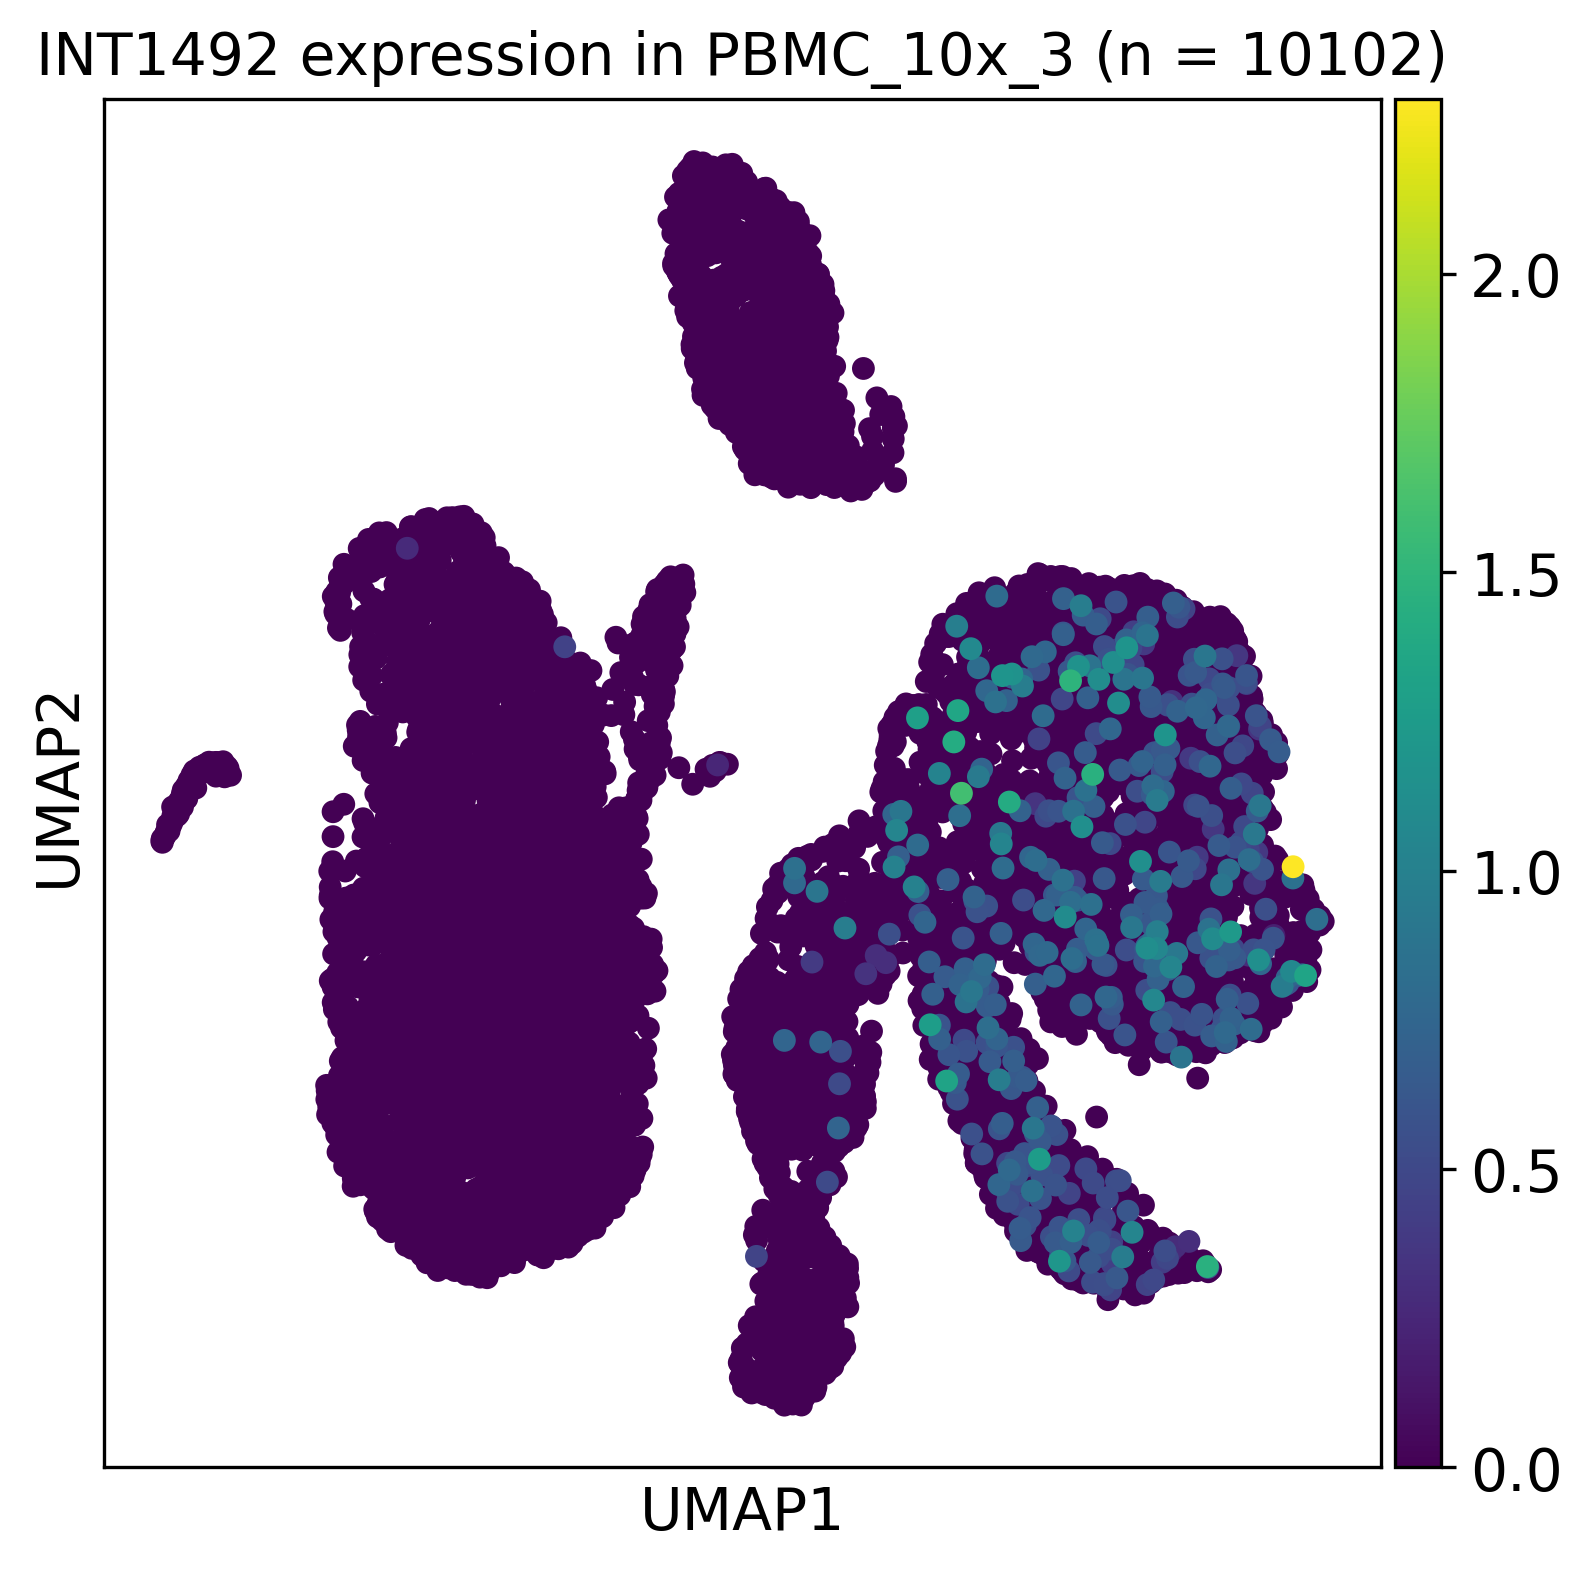
\includegraphics[width=0.45\textwidth]{images/isolatedDGEexamples/INT1492_PBMC_10x_3.png} &
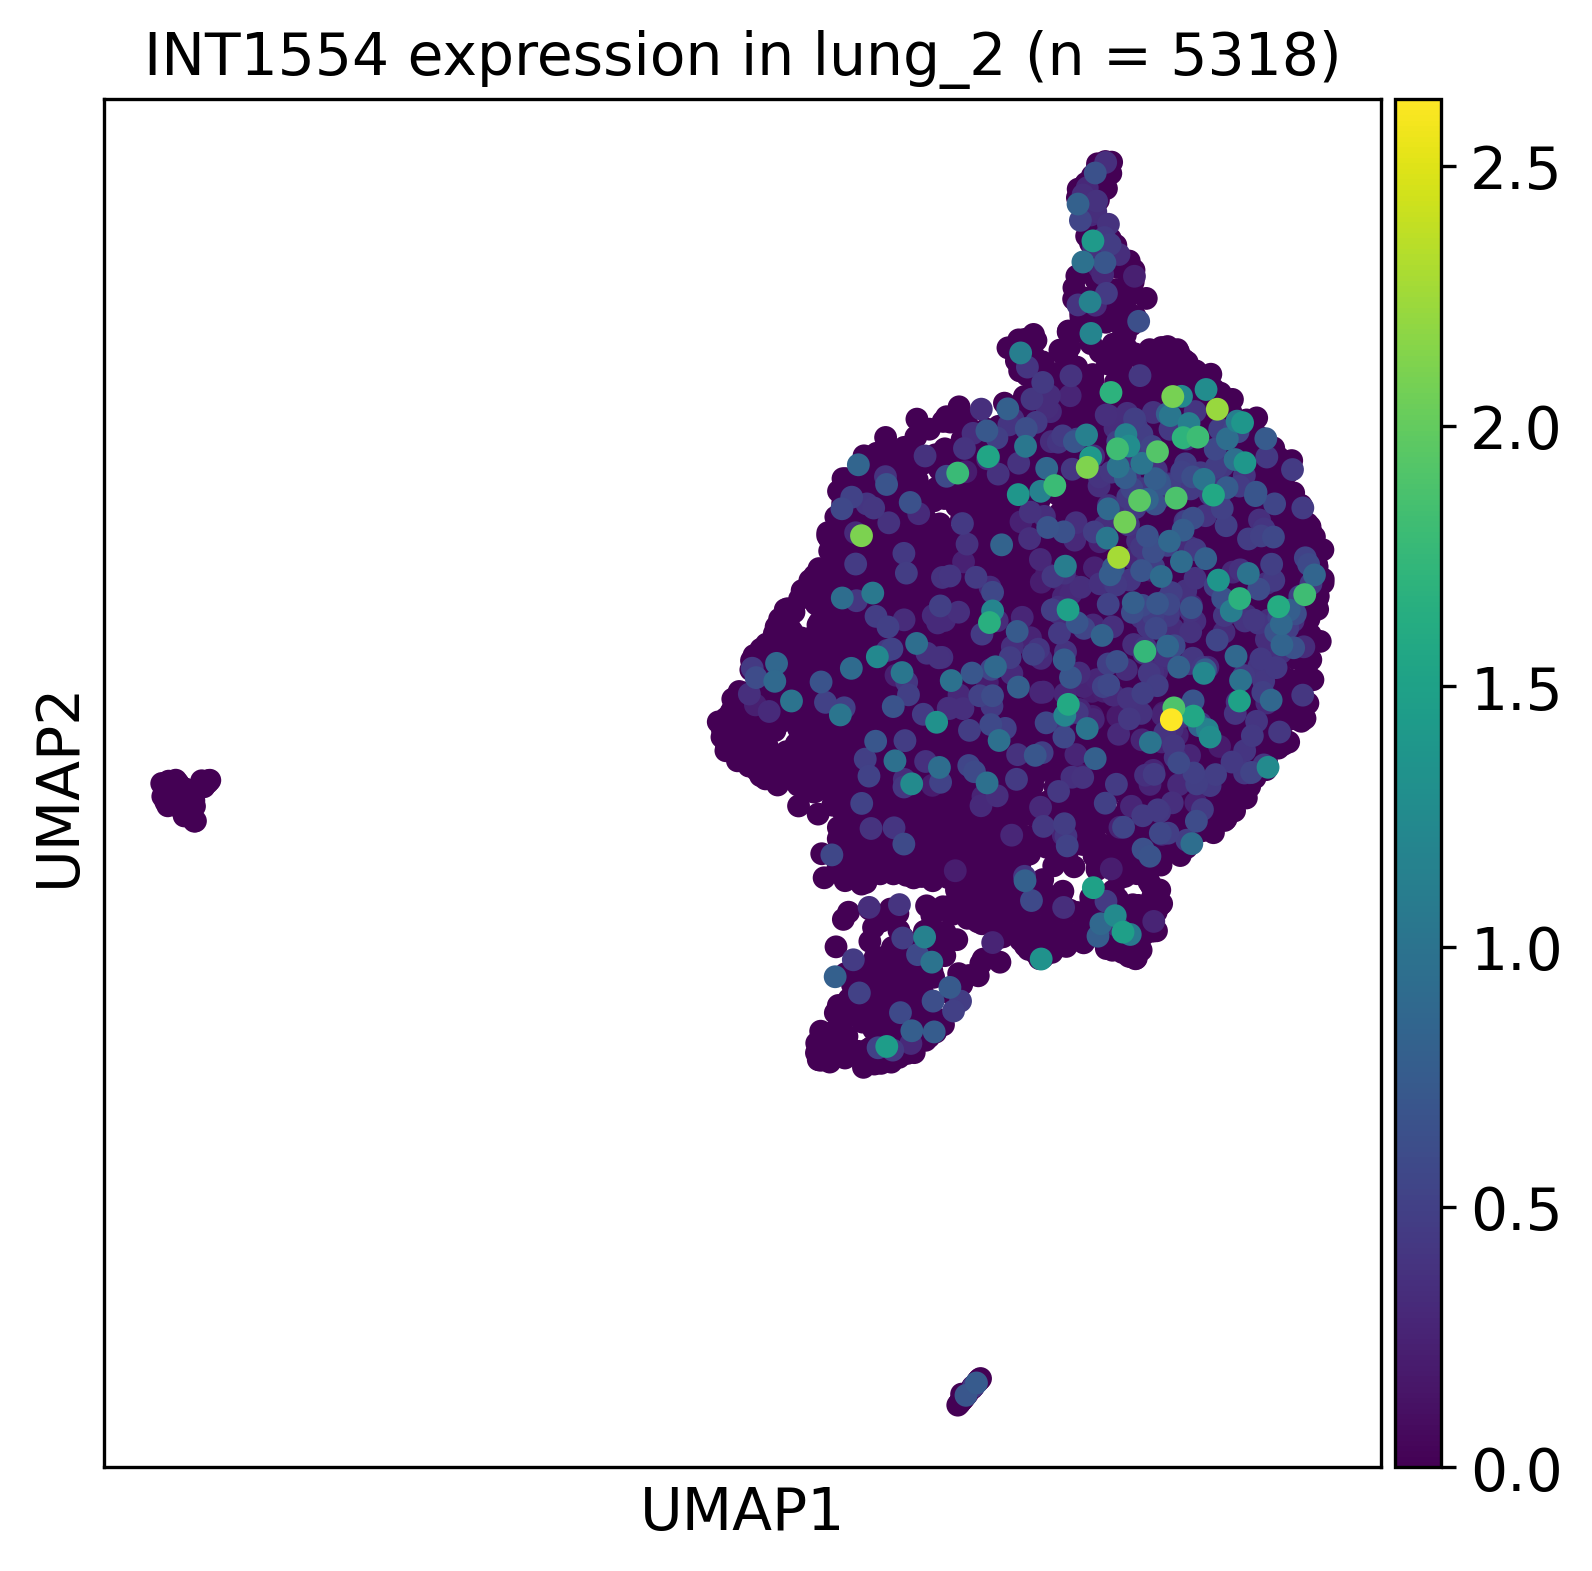
\includegraphics[width=0.45\textwidth]{images/isolatedDGEexamples/INT1554_lung_2.png} \\
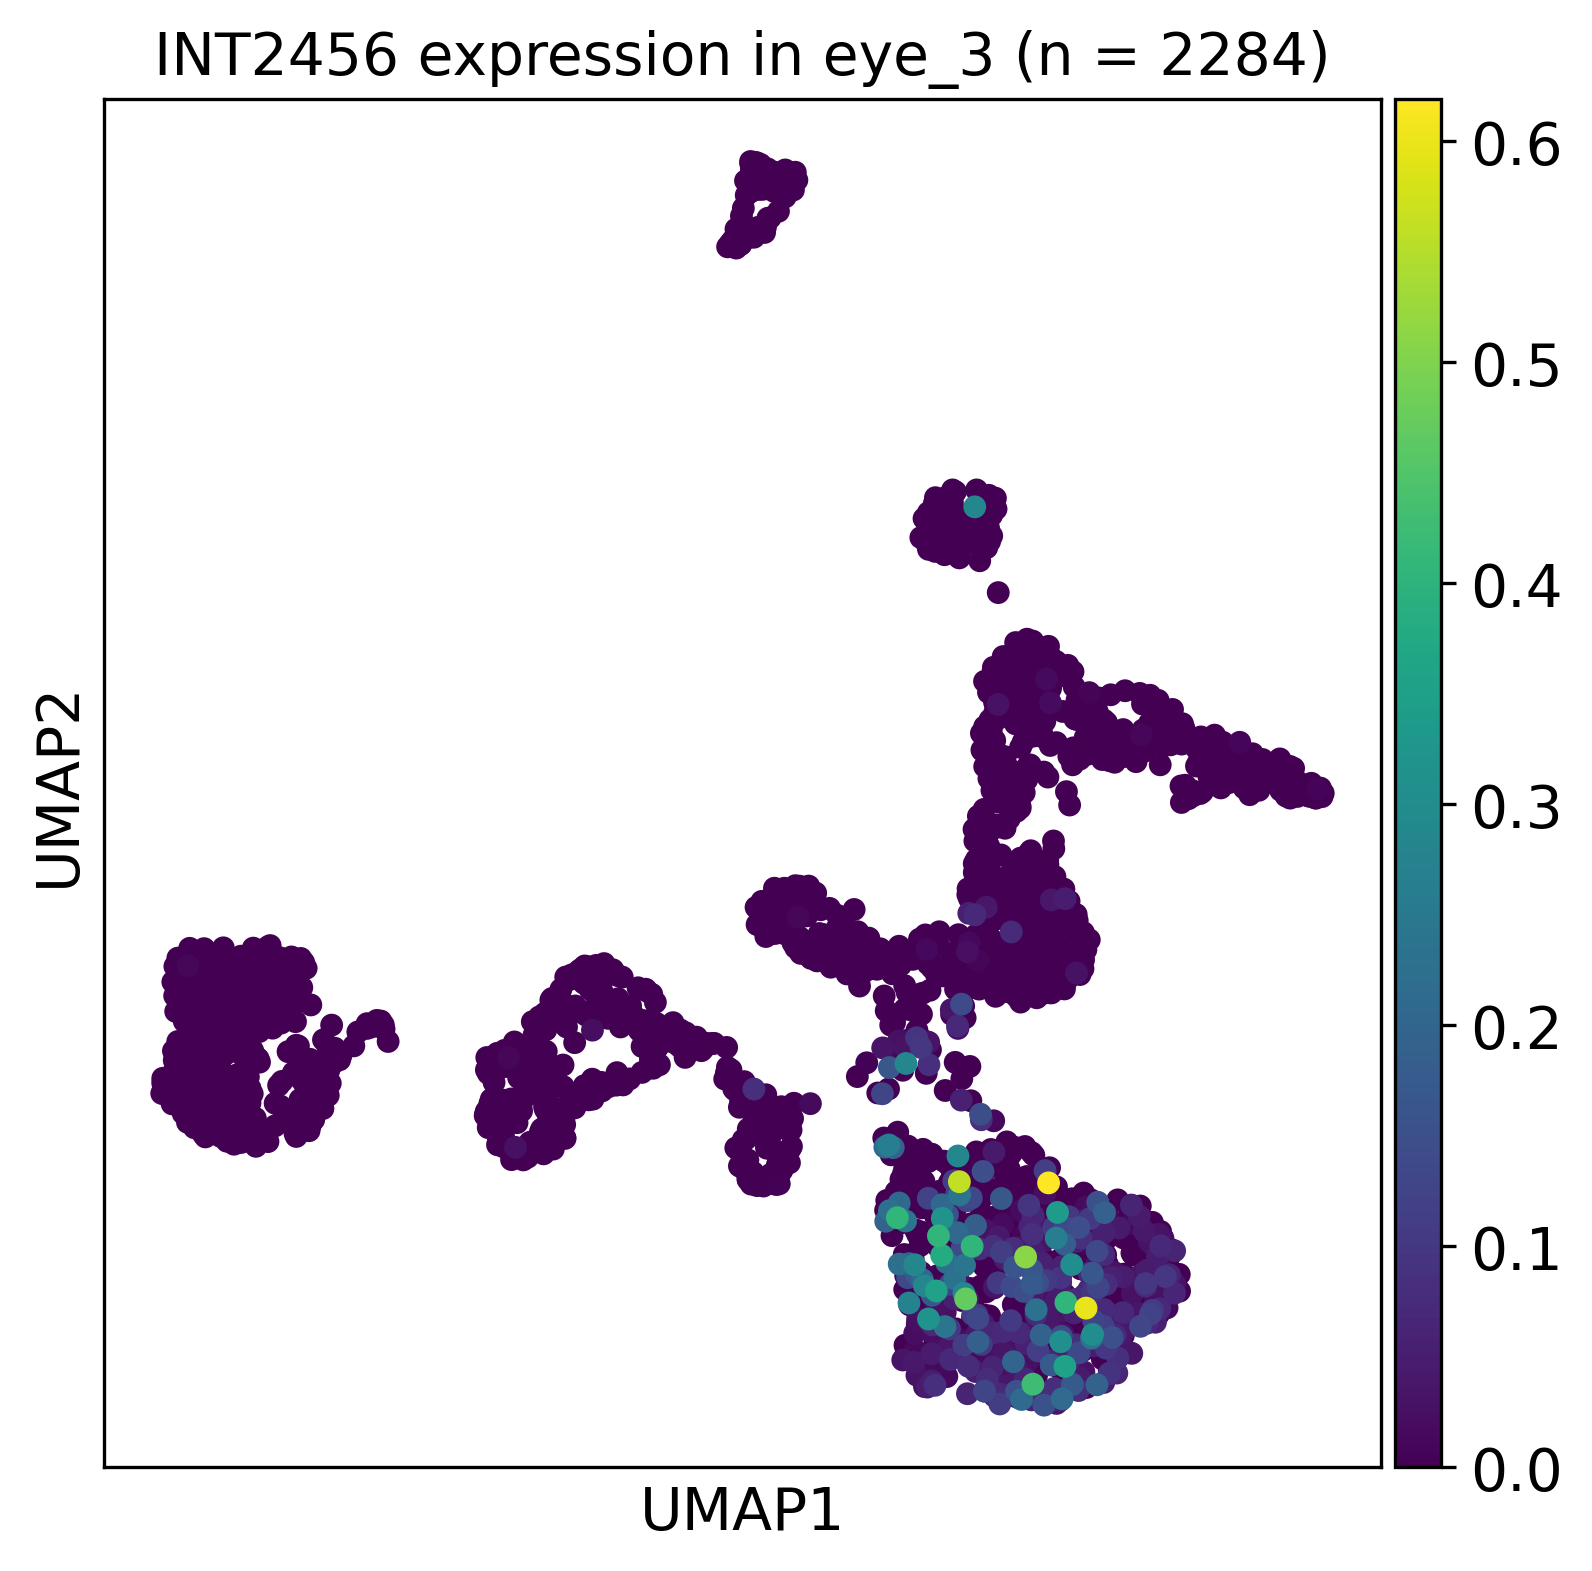
\includegraphics[width=0.45\textwidth]{images/isolatedDGEexamples/INT2456_eye_3.png} &
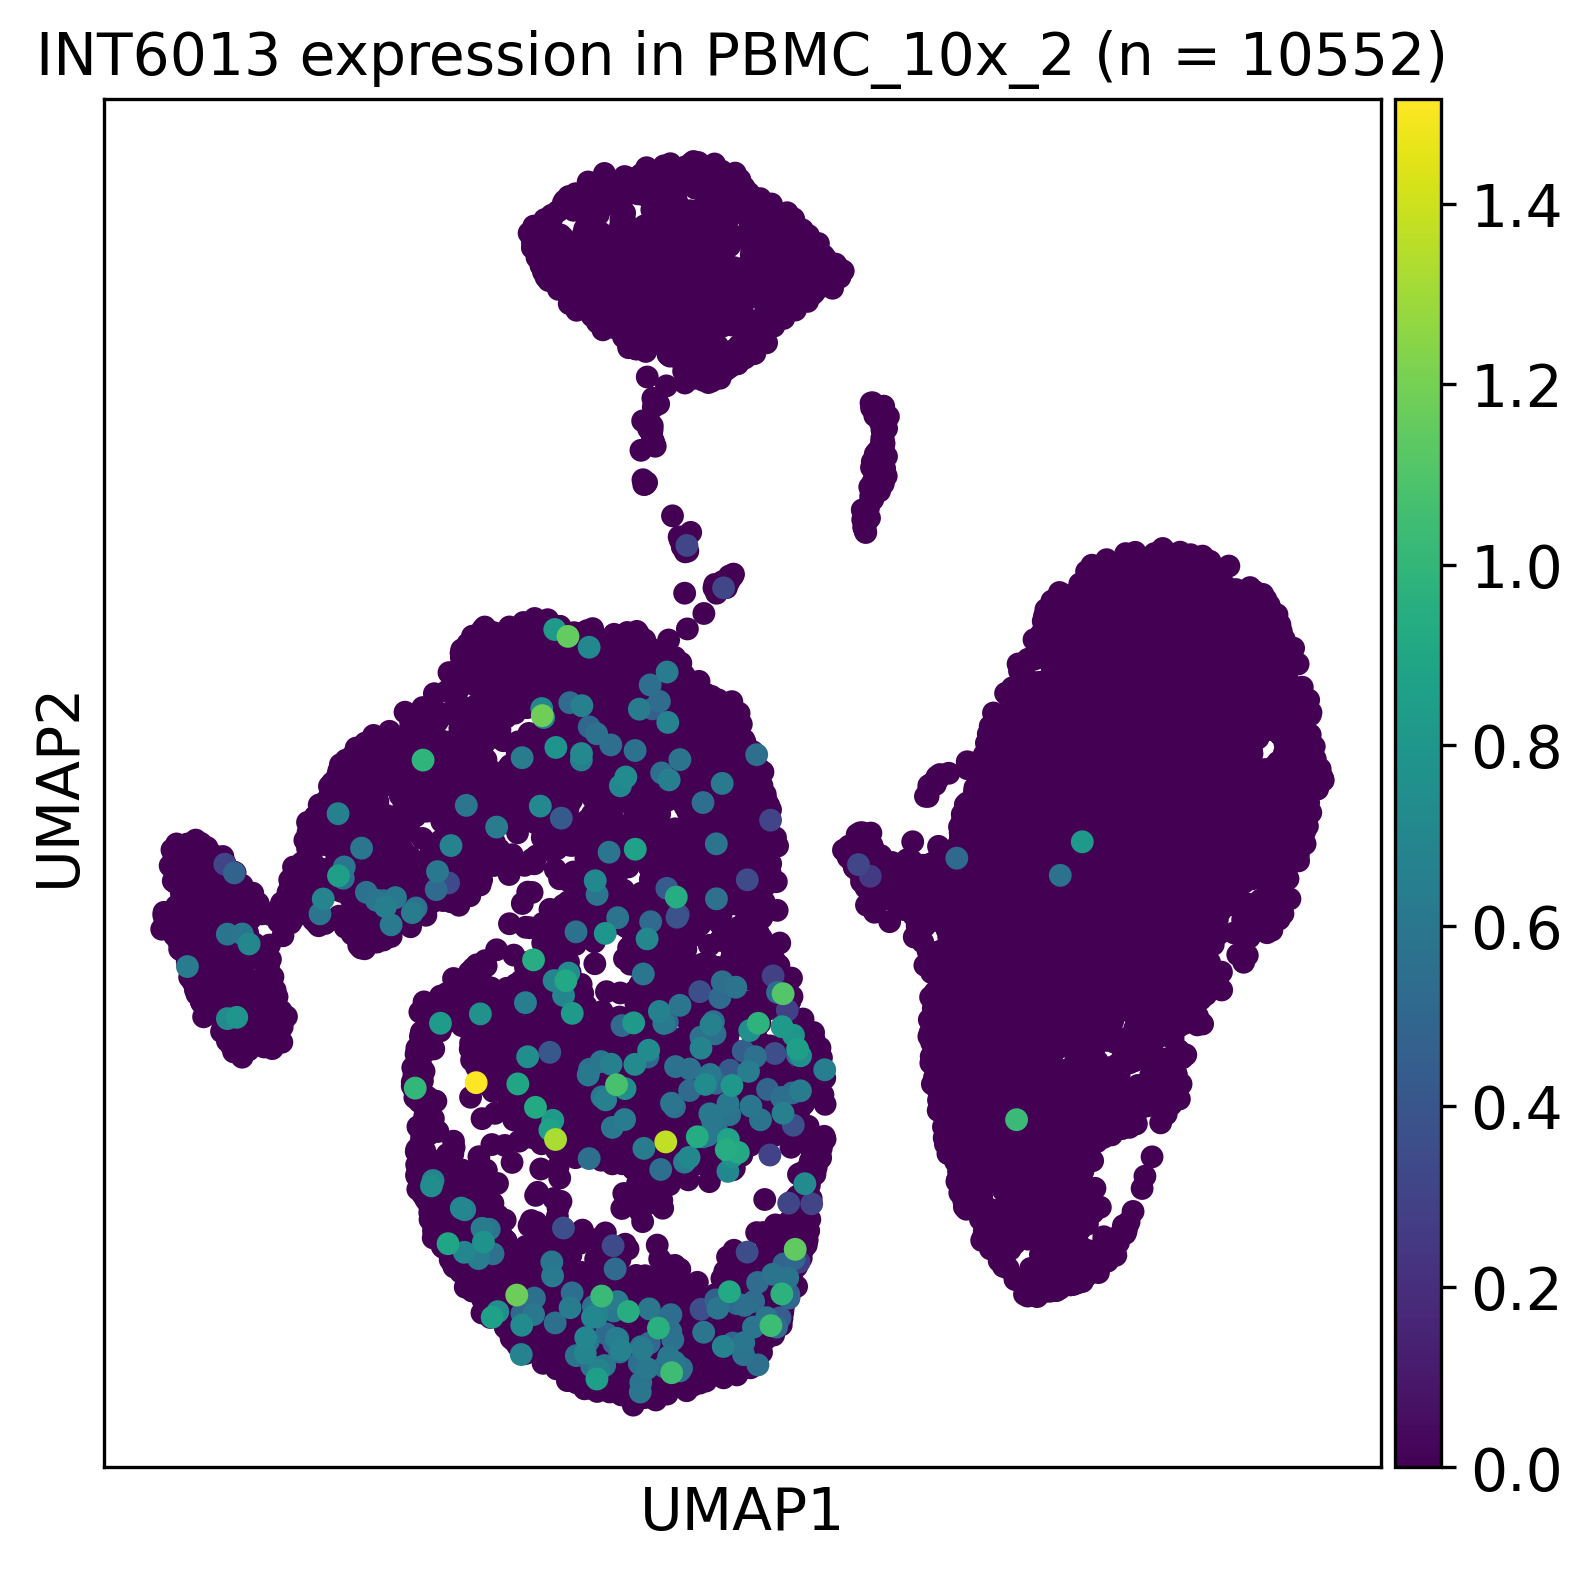
\includegraphics[width=0.45\textwidth]{images/isolatedDGEexamples/INT6013_PBMC_10x_2.png} \\
\end{tabular}
\caption{Examples of differentially expressed isolated intergenic regions.}
\label{fig:isolatedDGE}
\end{figure}

\paragraph{AT-rich regions}

AT-rich regions (here defined as 10 consecutive A's or T's, allowing one 'error', i.e. other nuucleotide)
were looked upstream of the isolated intergenic regions, and the first hits were reported.

34 of the intergenic regions overlapped such AT rich regions, the distances from other isolated intergenic regions to such AT-rich regions varied,
with mean 748 and median 283, the histogram can be seen in the Figure \ref{fig:distancesATrich}.

\begin{figure}
  \centering
  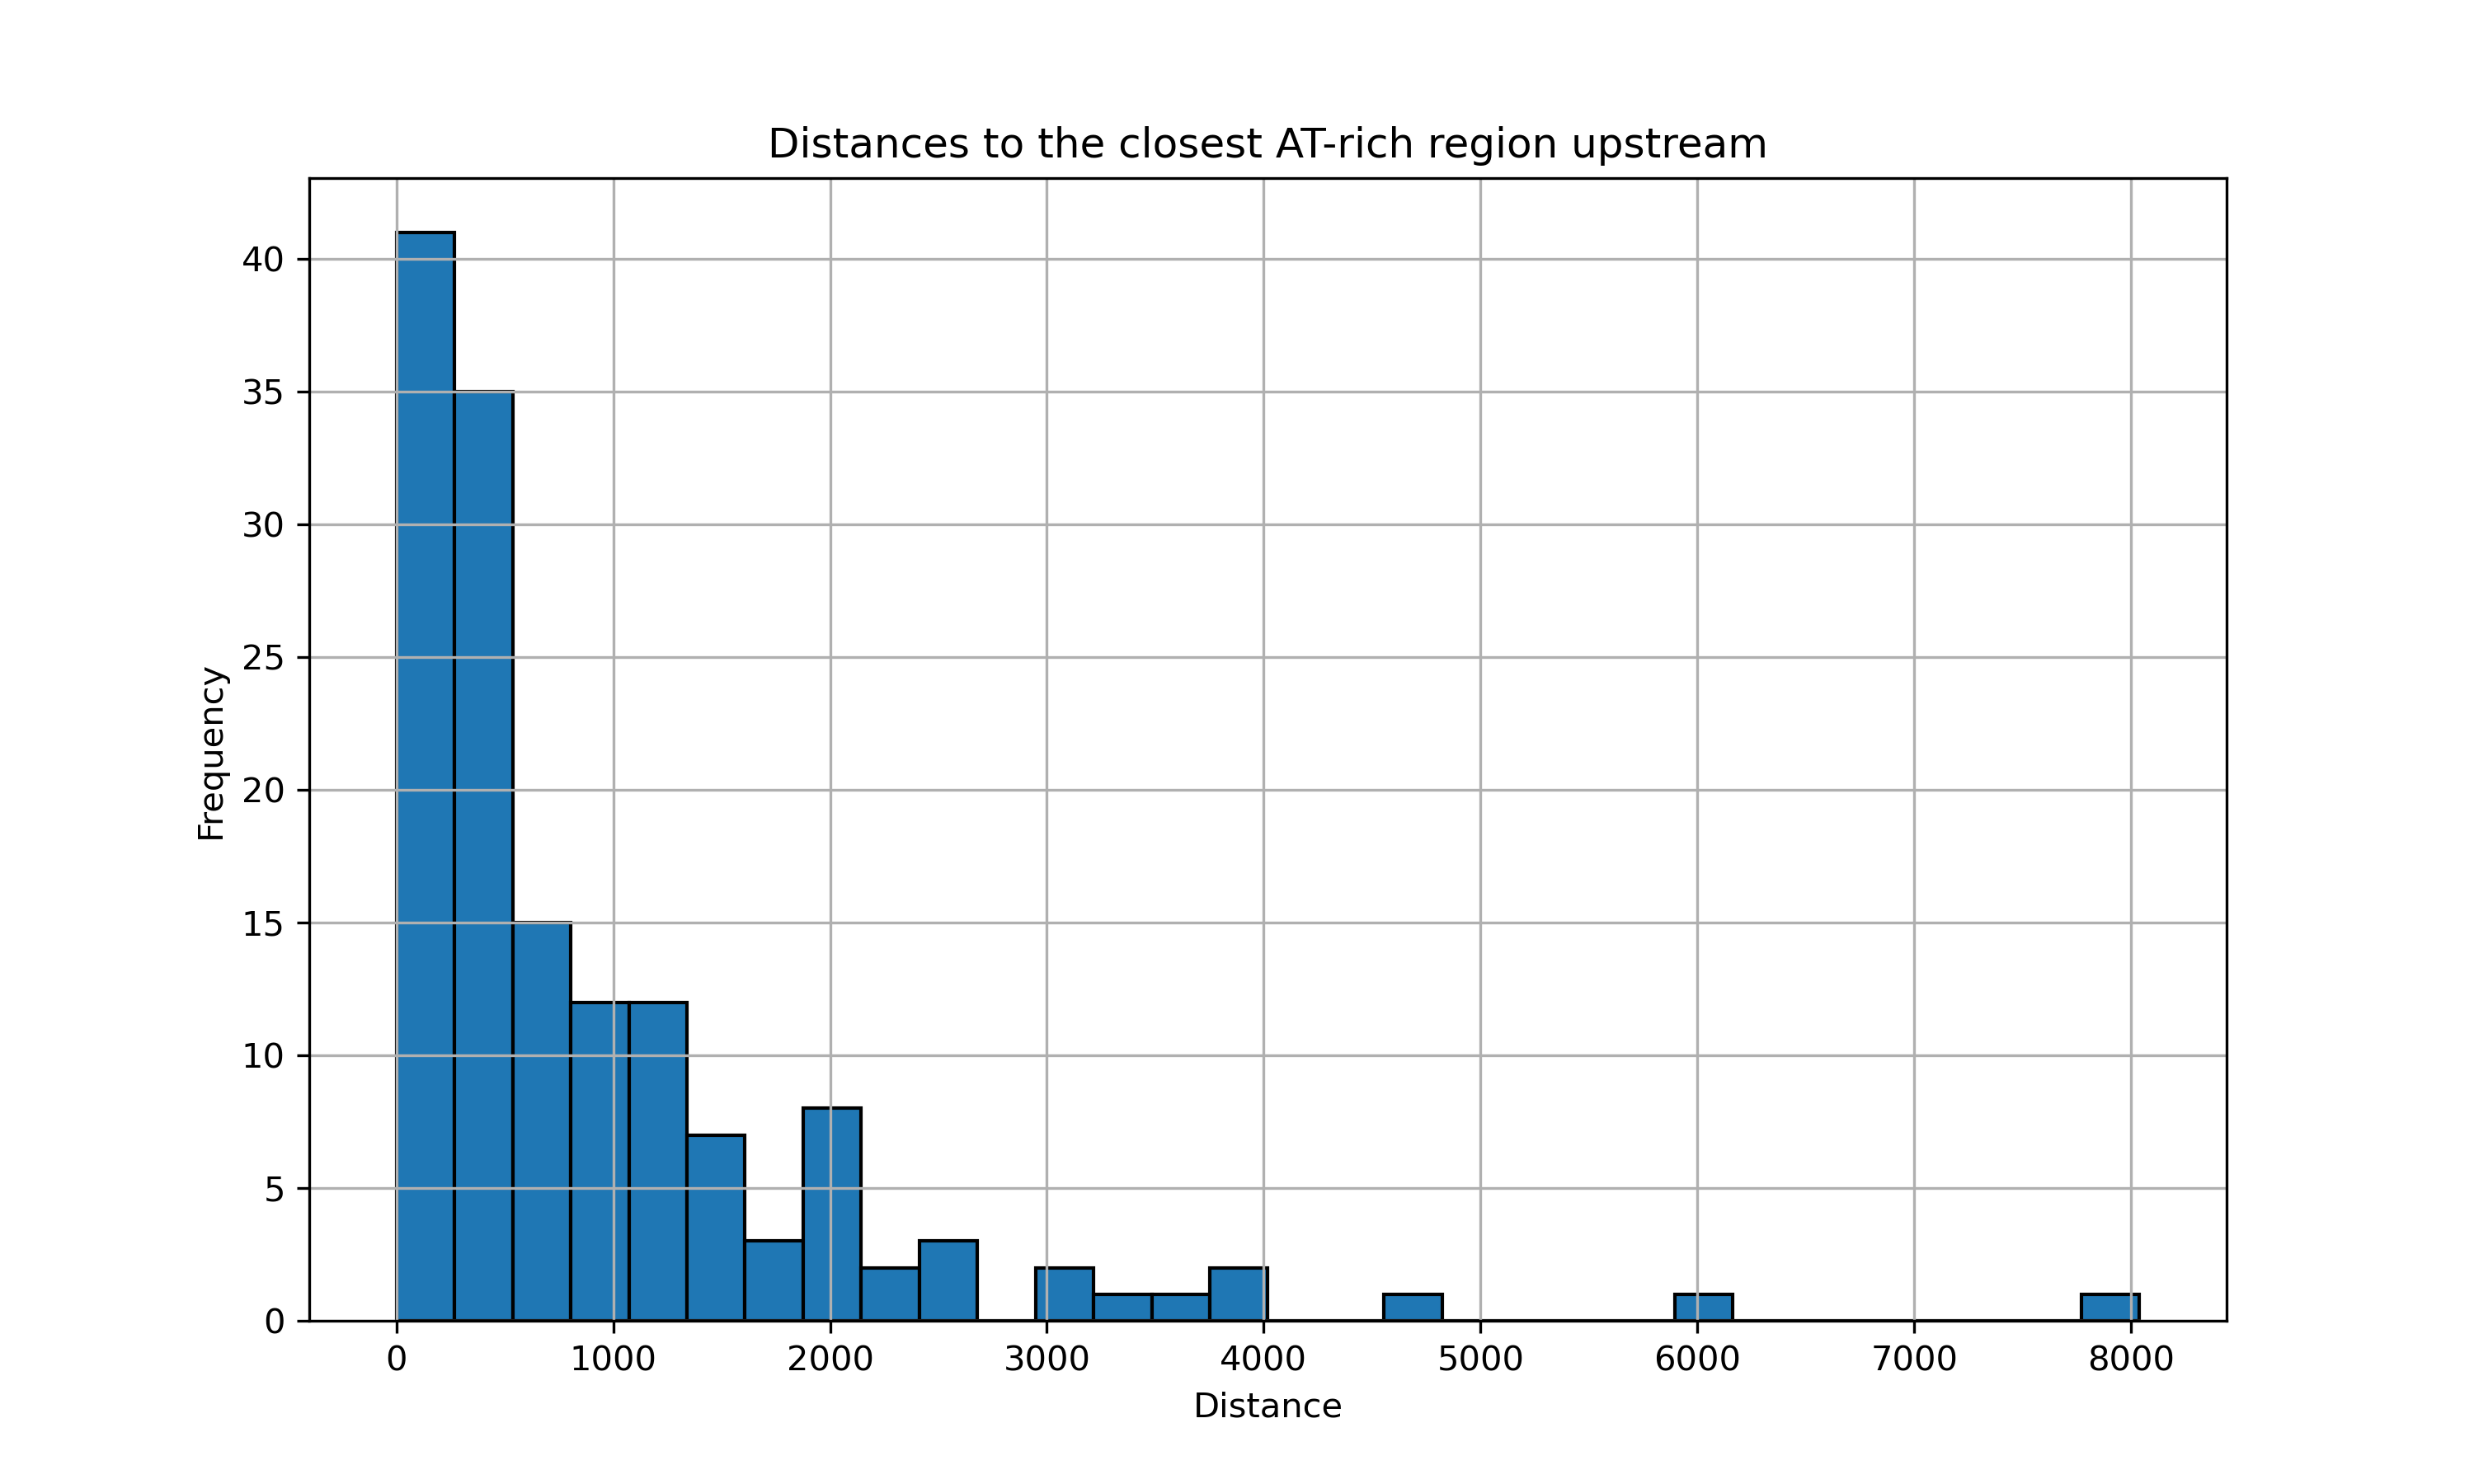
\includegraphics[width=\linewidth]{images/histogramATrich.png}
  \caption{Distances from isolated intergenic regions to closest AT-rich region upstream
  (if intergenic regions overlaps with AT-rich region, distance is set to 0)}
  \label{fig:distancesATrich}
\end{figure}

\paragraph{Open chromatin}

Open chromatin regions could provide additional evidence of transcriptional activity, if found in the upstream regions.
However, to be more specific, distances to the closest genes should also be found and compared, 
as those open chromatin sites upstream not necessarily are related to our intergenic regions, if there are other genes upstream,
they could be the cause for this.

The distances to open chromatin sites was found for each intergenic regions 




\iffalse

Firstly, to check if the intergenic regions contain any biologically meaningfull information,
for each sample cells were clustered based only on those intergenic samples.
As can be seen in some provided examples in Figure \ref{fig:intergenicClustering},
clustering can be seen in this case and it roughly corresponds to the clustering using standard ('10x') annotation.
This shows that biologically meaningful information is indeed present in those intergenic regions,
Hence, further analysis were performed on those intergenic regions.

The intergenic regions from all samples were combined into one list, resulting in a list of 13667 entries.
For each region several metrics were calculated, including mean CPM (counts per million) per sample,
the number of samples in which this region was detected, conservation score.
Additionally it was checked if those regions overalap with any genes predicted by gene predictions tools,
also, closest genes on the same and opposite strands (and distances from them) were found.
The list was filtered based on the numer of samples the region was detected, allowing only those regions that are detected in all
blood, brain, eye, or lung samples (with the exception for PBMC samples,
for them more permissive filtering was applied, allowing those entries that were detected only by one sequencing protocol as well,
i.e. it could be detected in all 'PBMC\_10x samples' or all 'PBMC\_indrops samples').
This resulted in a filtered list of 2590 intergenic regions.

Since the filtered list still remained huge, additional filtering criterions were applied:
\begin{itemize}
  \item \textbf{Conservation scores.} Since the conservation scores are not strand specific,
  it makes no sense to filter out directly by the conservation score, because in the case there is other gene on the opposite strand
  of defined region, the high conservation score could be induced by this other gene.
  However, if there are no overlapping genes, high conservation score of an intergenic region could suggest that it might have some function.
  Therefore, a group of possibly biologically meaningful locations were extracted by filtering those genes that have high conservation score
  (threshold was set to 0.6) and do not overlap with any known genes (from the ncbi or genecode references).
  \item \textbf{Gene predictions tools.} There are tools that predict genes based on the genomic sequence.
  Such predictions (if overlapping with defined intergenic regions) would support the claim that
  those (overlapping) intergenic regions are not noise, especially if the intergenic peaks would overlap with 3' ends of predicted genes.
  \item \textbf{Intergenic region specificity.} In the case the reads from specific regions are present only in one cell group,
  the biological origin of these reads are very likelly.
  Such specific regions can be noticed using differential gene expression analysis,
  i.e. checking how gene (or in our case, intergenic region) expression varies between different cell types.
  \item \textbf{ATAC data.} ATAC data can show open chromatin regions, which are typically associated with active transcription.
  If the intergenic regions overlap with open chromatin regions, this could provide additional evidence that reads from this region is not noise.
  \item \textbf{Correlations with nearby genes.} If there exist correlations between the expression of the intergenic regions
  and expression of nearby genes, that could suggest that those regions are not noise and are involved in the same pathways as their neighbours.
\end{itemize}

In the following subsections I will explore genes filtered by those strategies separatelly.

\begin{figure}[htbp]
    \centering
    \begin{subfigure}{0.45\textwidth}
        \centering
        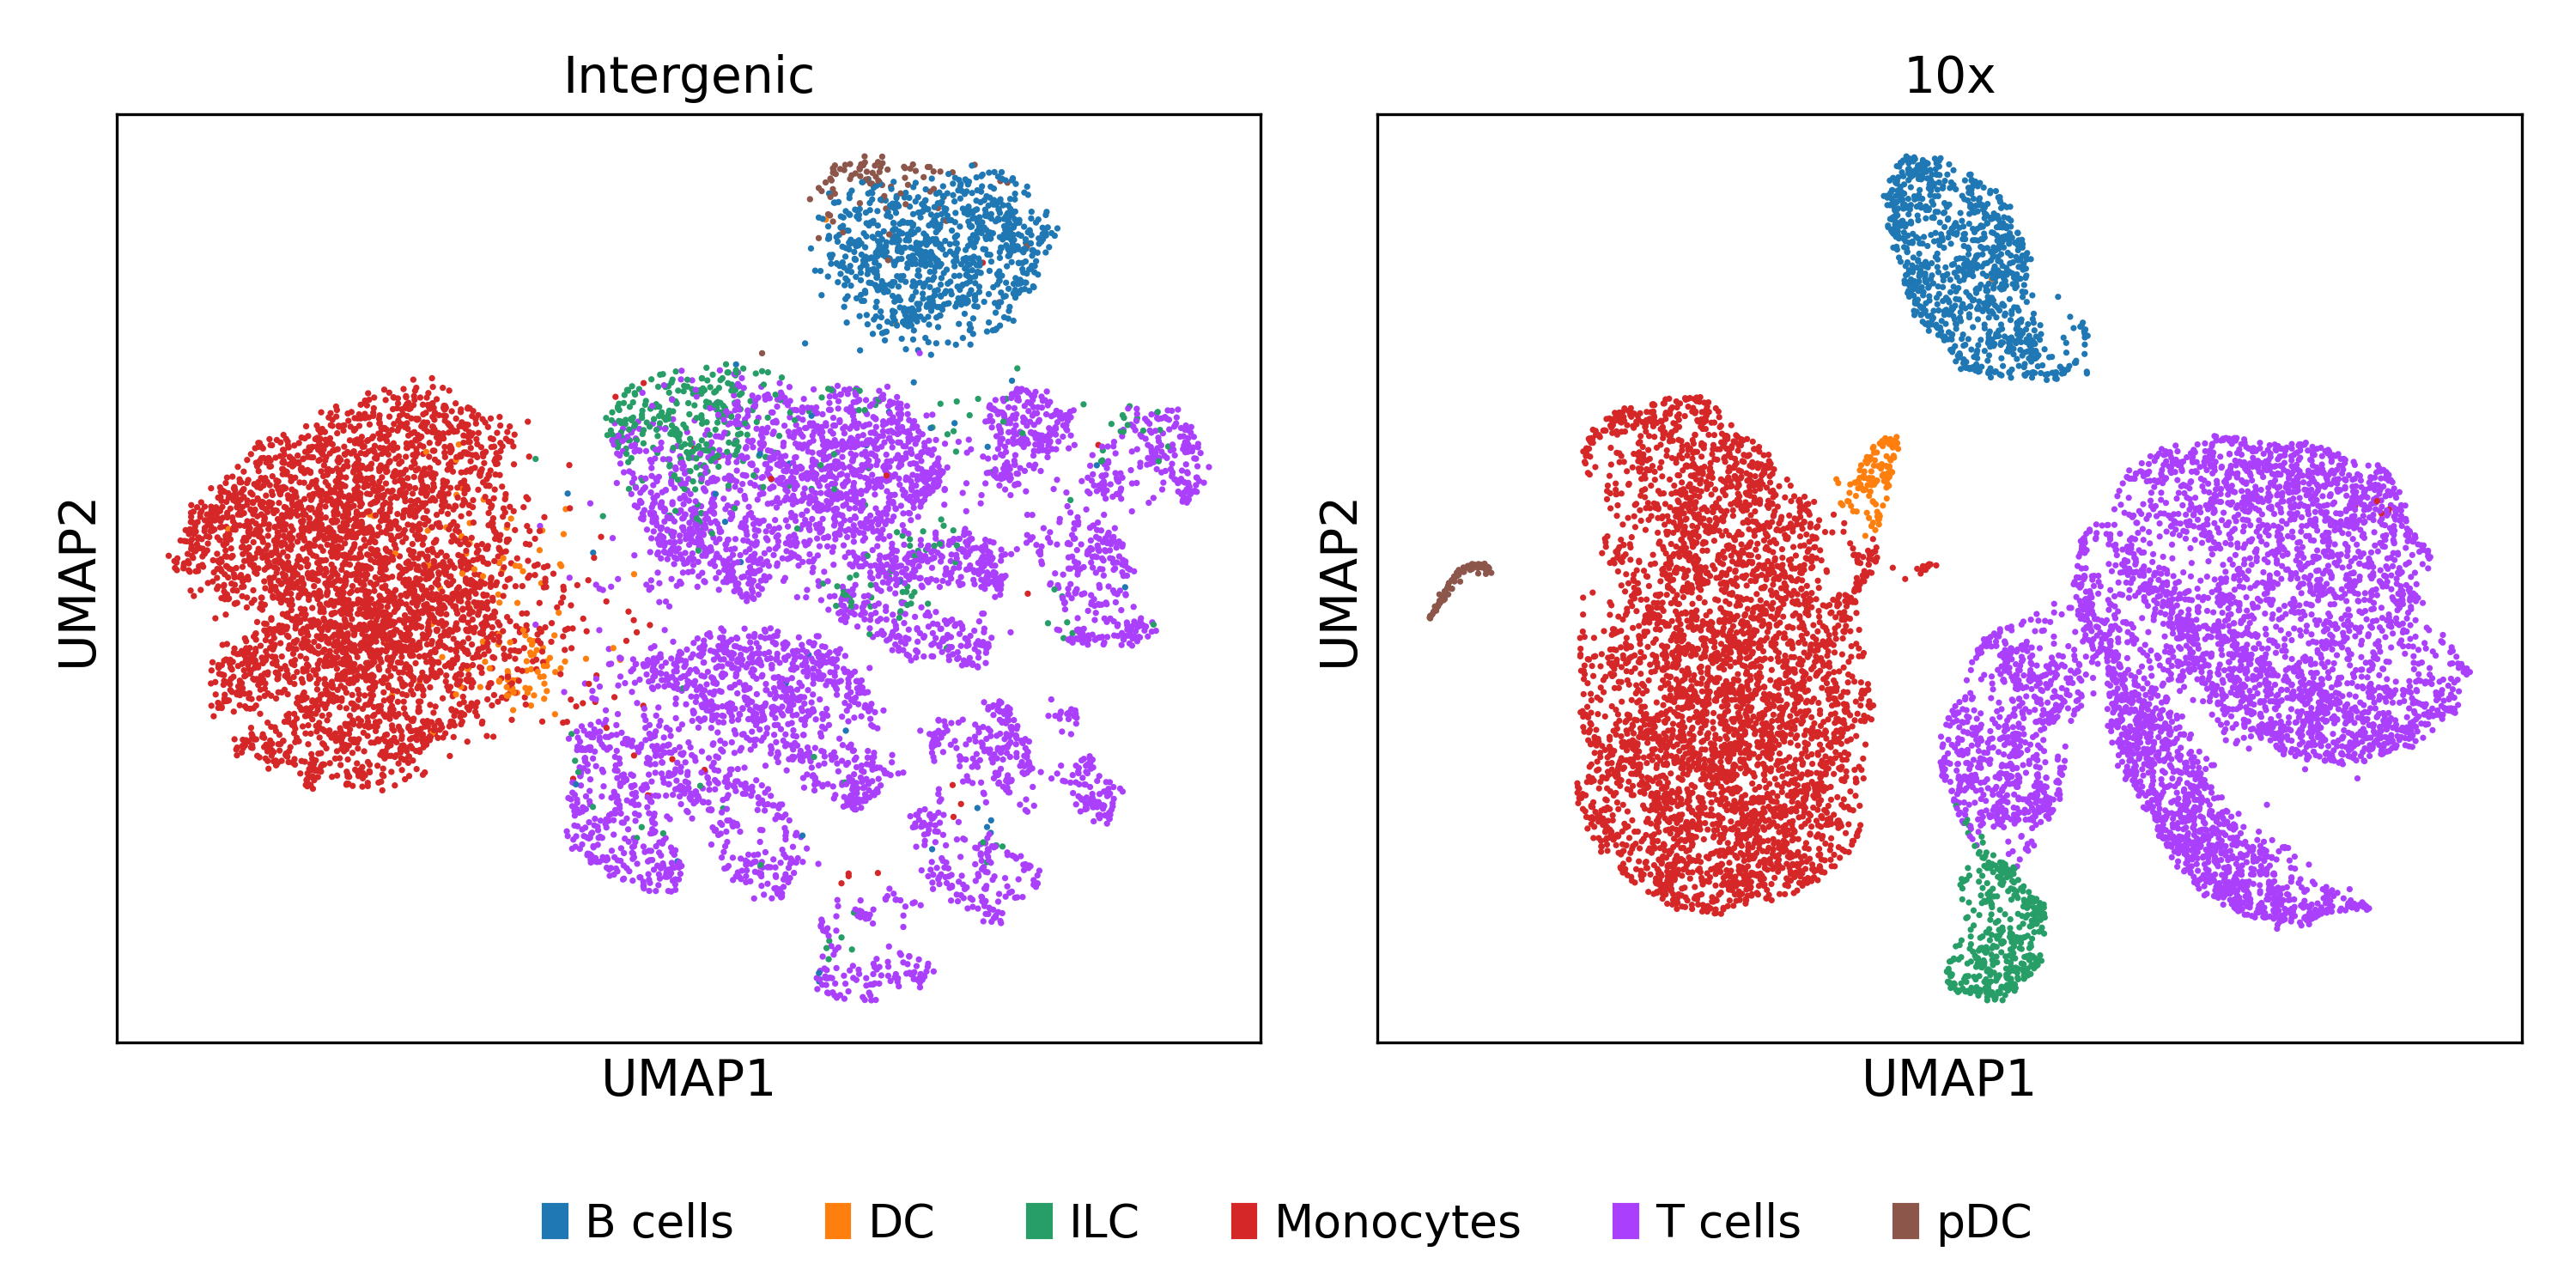
\includegraphics[width=\textwidth]{images/umaps/intergenic_10x_pbmc10x3.png}
        \caption{10x PBMC 3}
    \end{subfigure}
    \hfill
    \begin{subfigure}{0.45\textwidth}
        \centering
        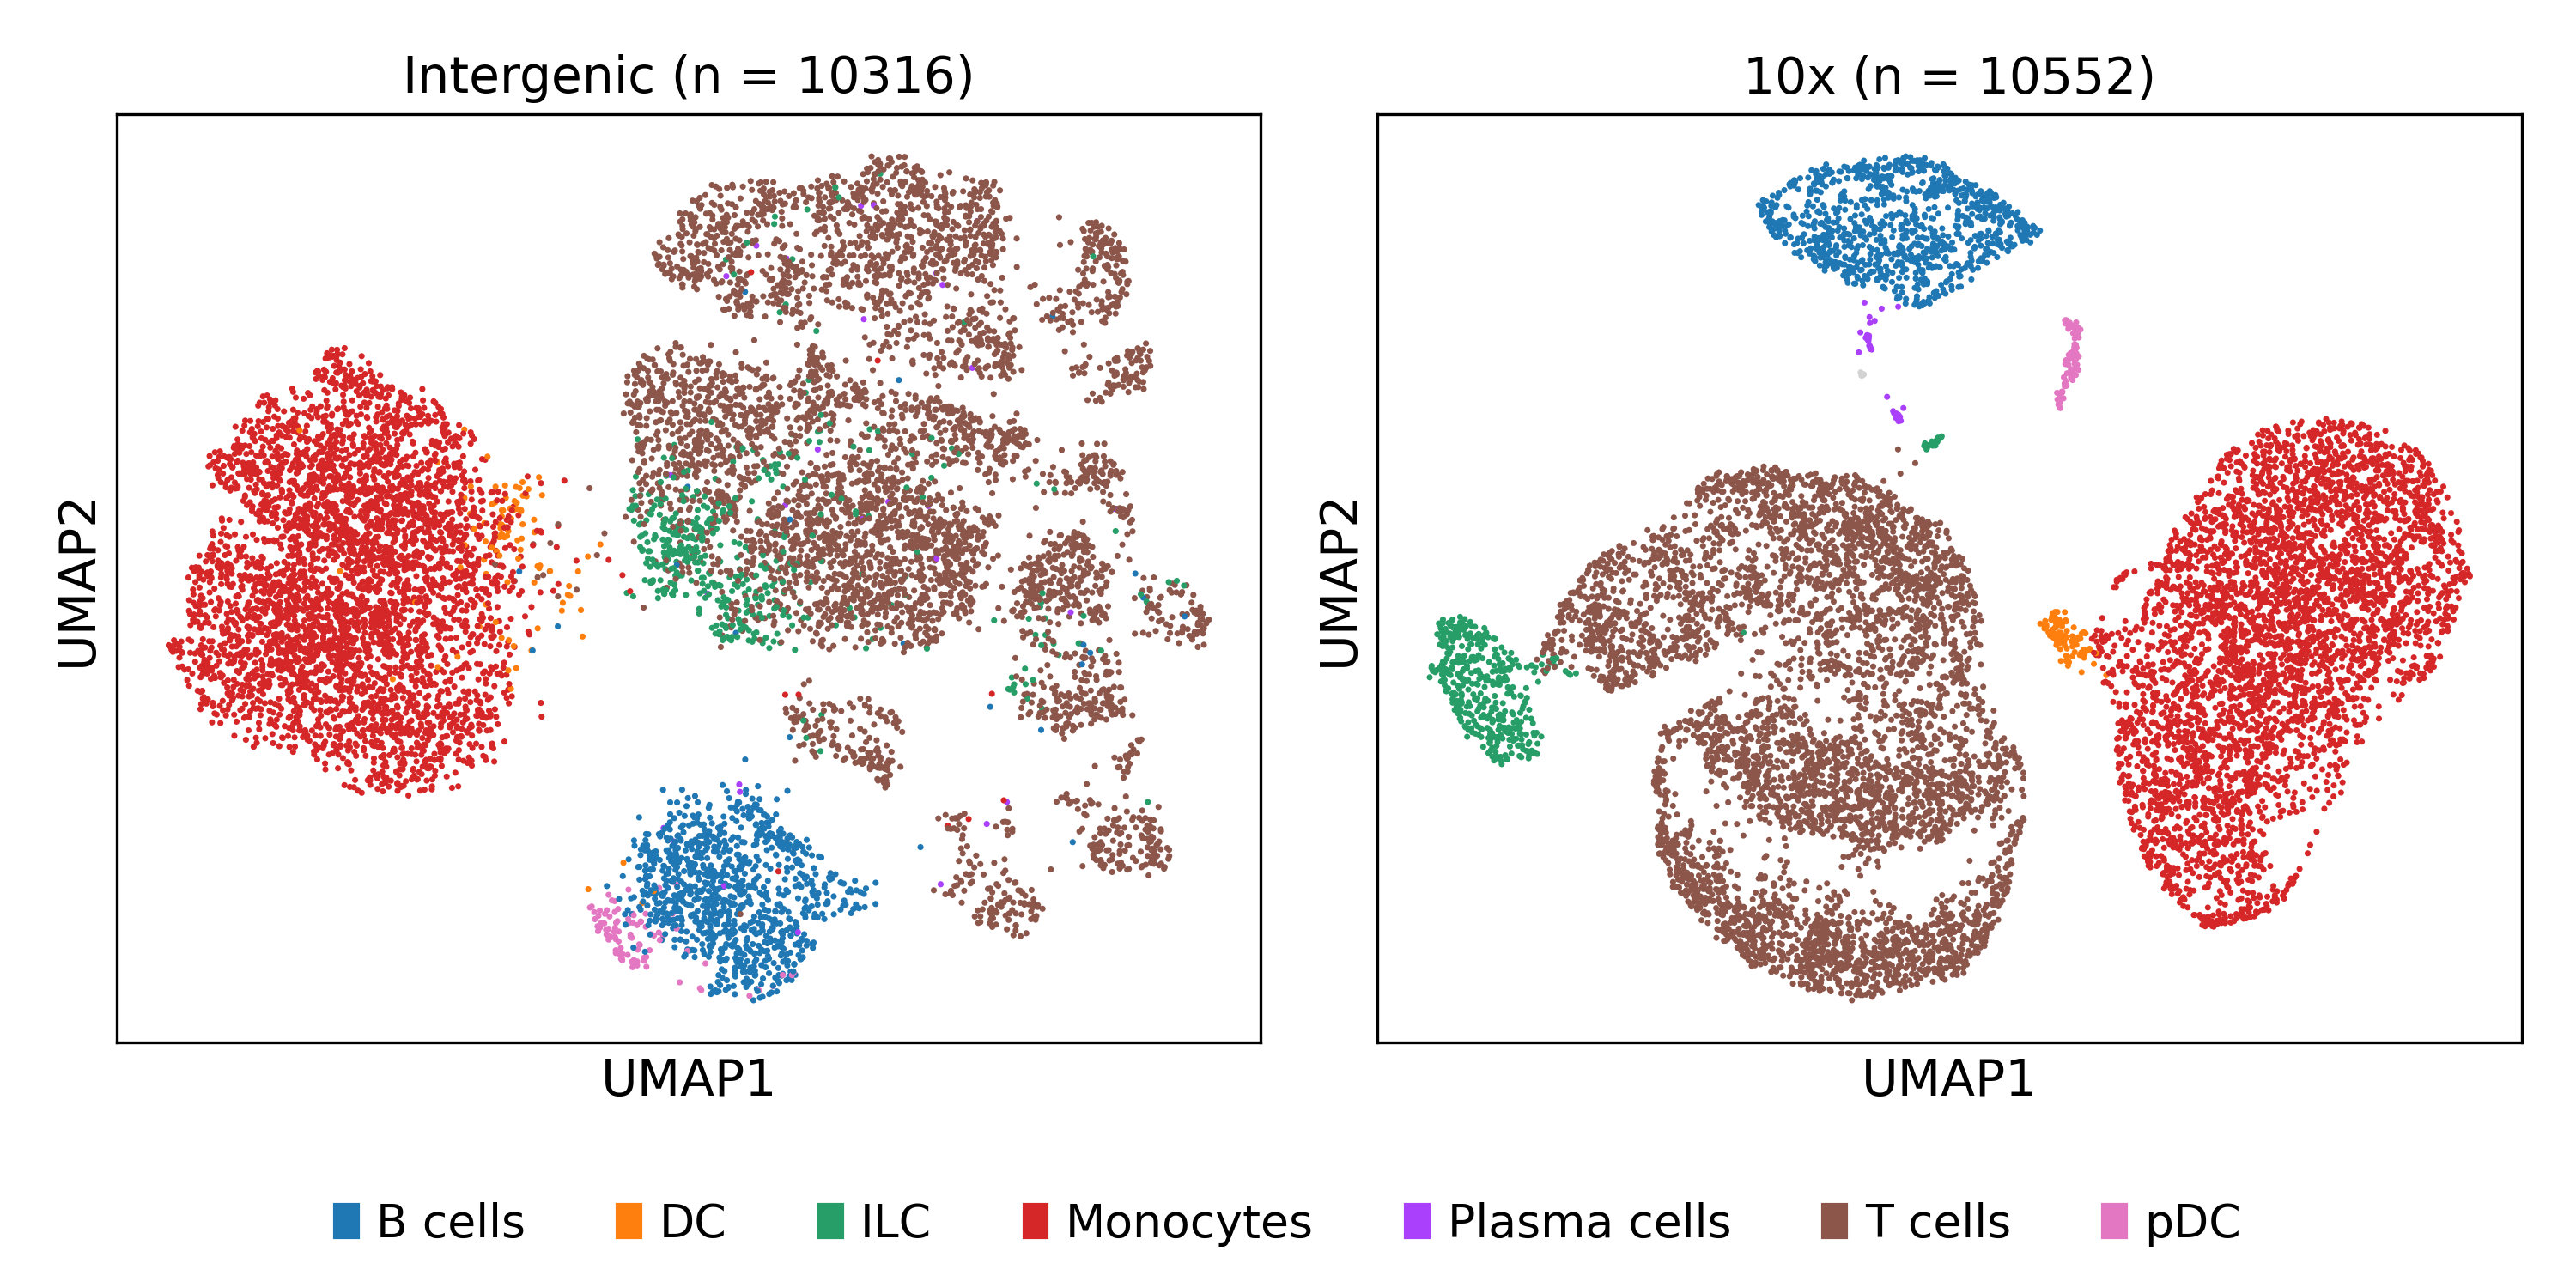
\includegraphics[width=\textwidth]{images/umaps/intergenic_10x_pbmc10x2.png}
        \caption{10x PBMC 2}
    \end{subfigure}
    \vspace{0.5em}
    \begin{subfigure}{0.45\textwidth}
        \centering
        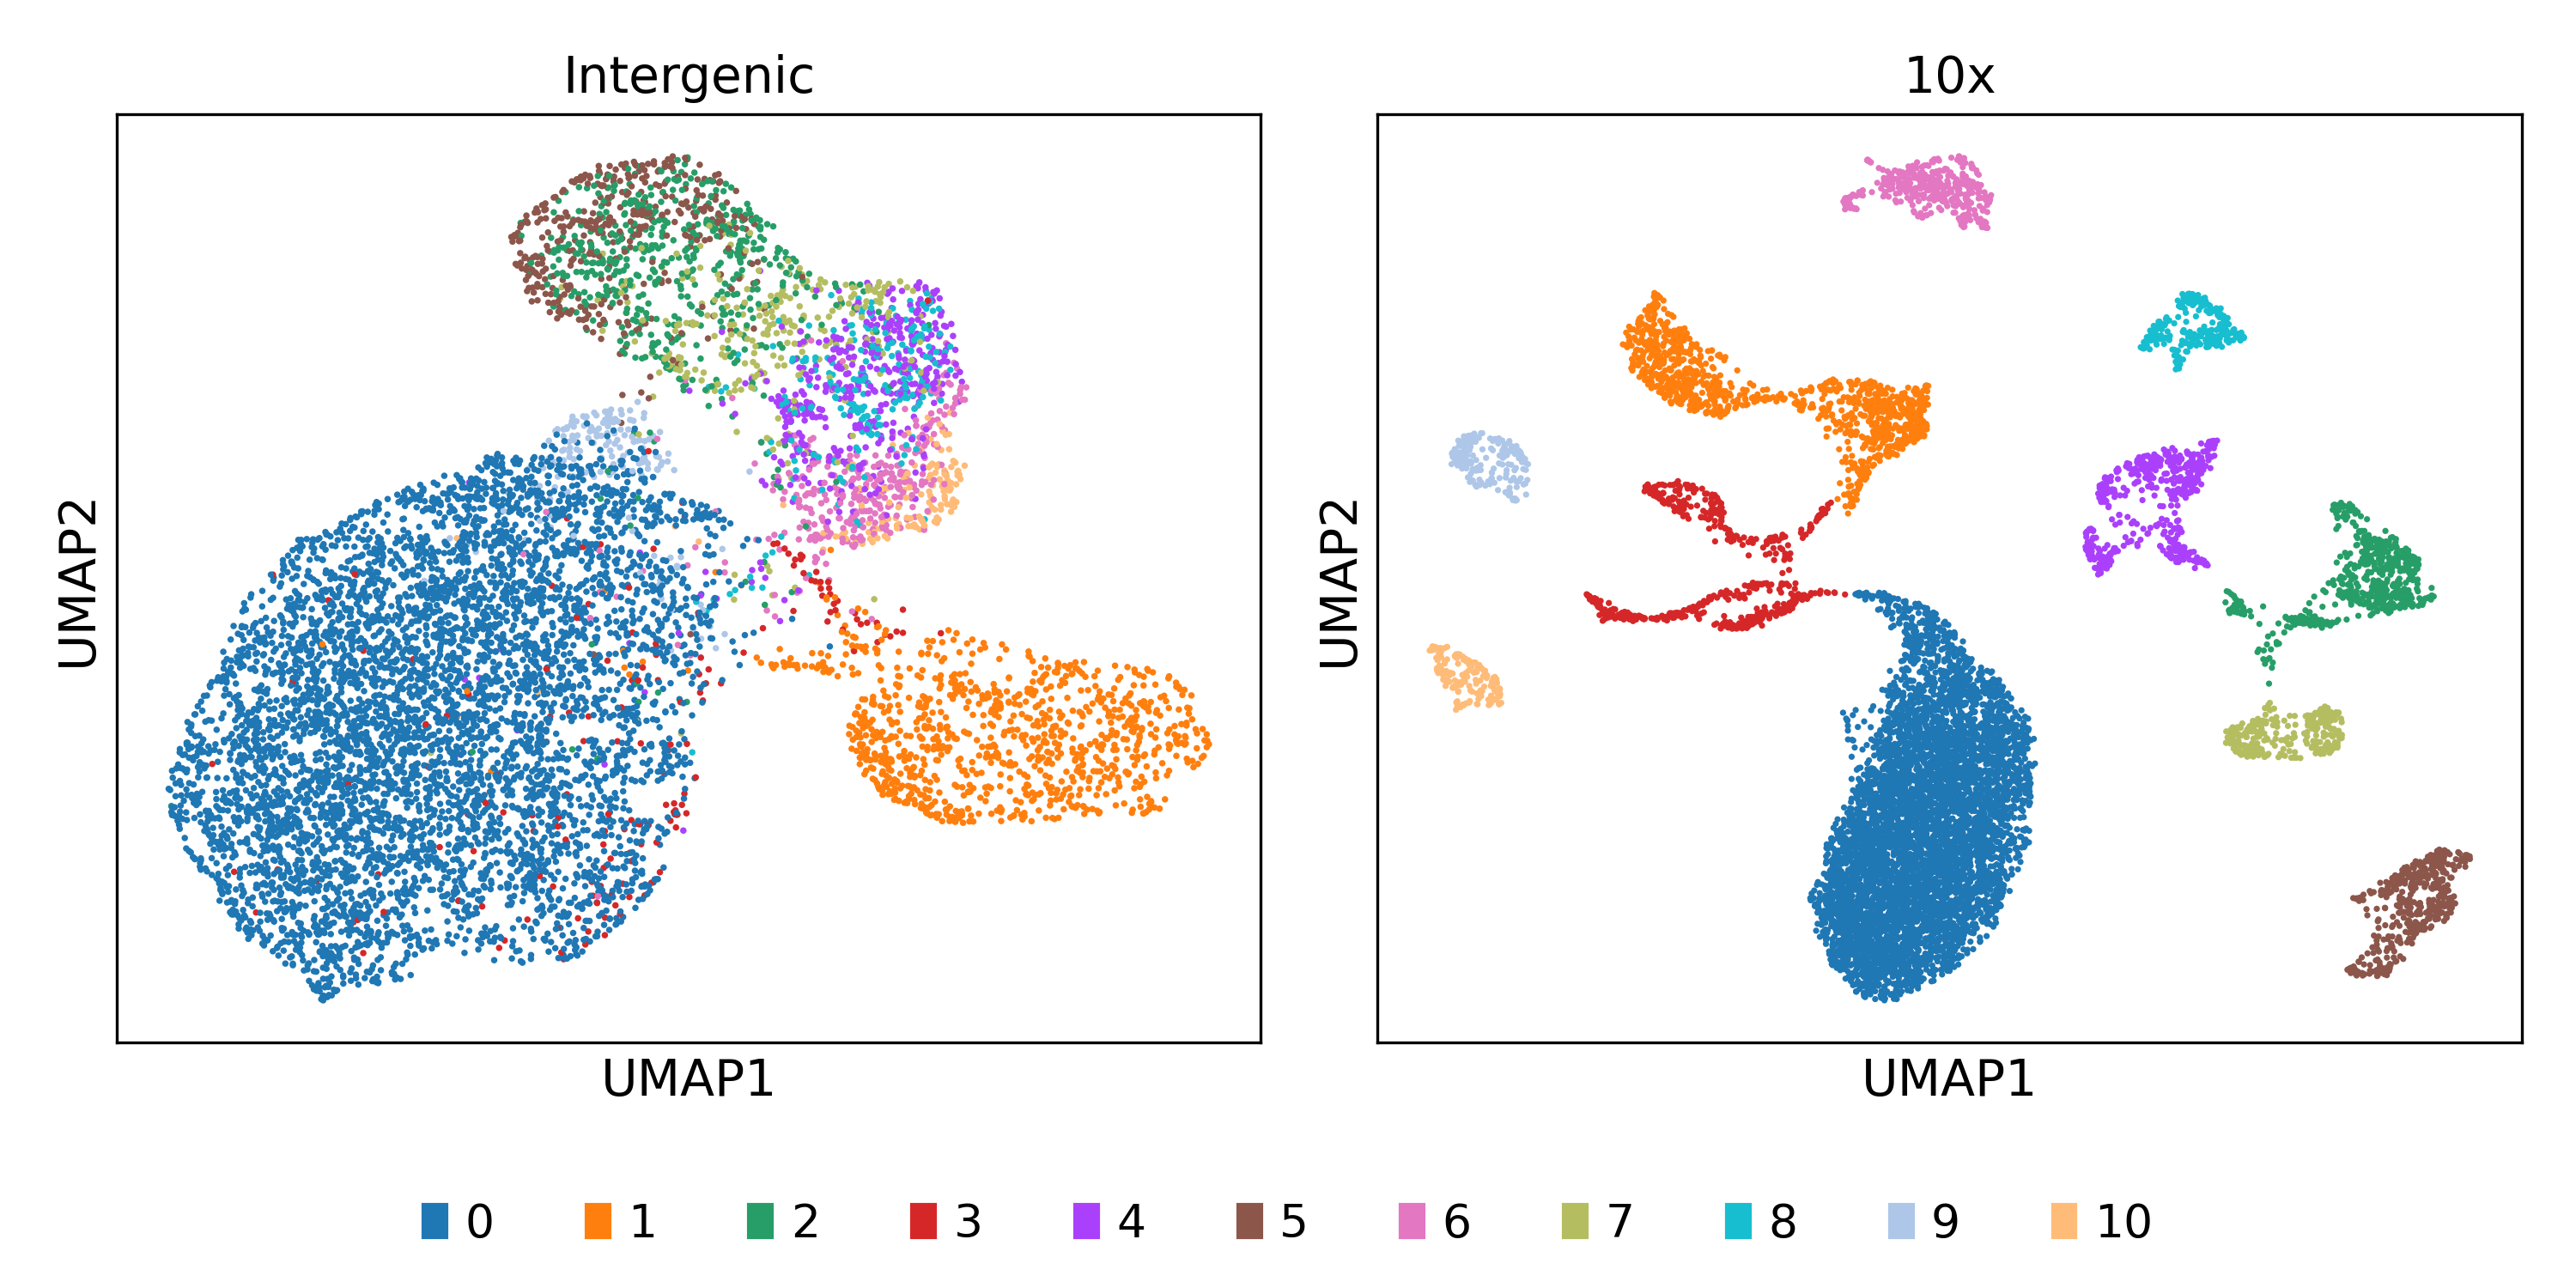
\includegraphics[width=\textwidth]{images/umaps/intergenic_10x_eye.png}
        \caption{eye}
    \end{subfigure}
    \hfill
    \begin{subfigure}{0.45\textwidth}
        \centering
        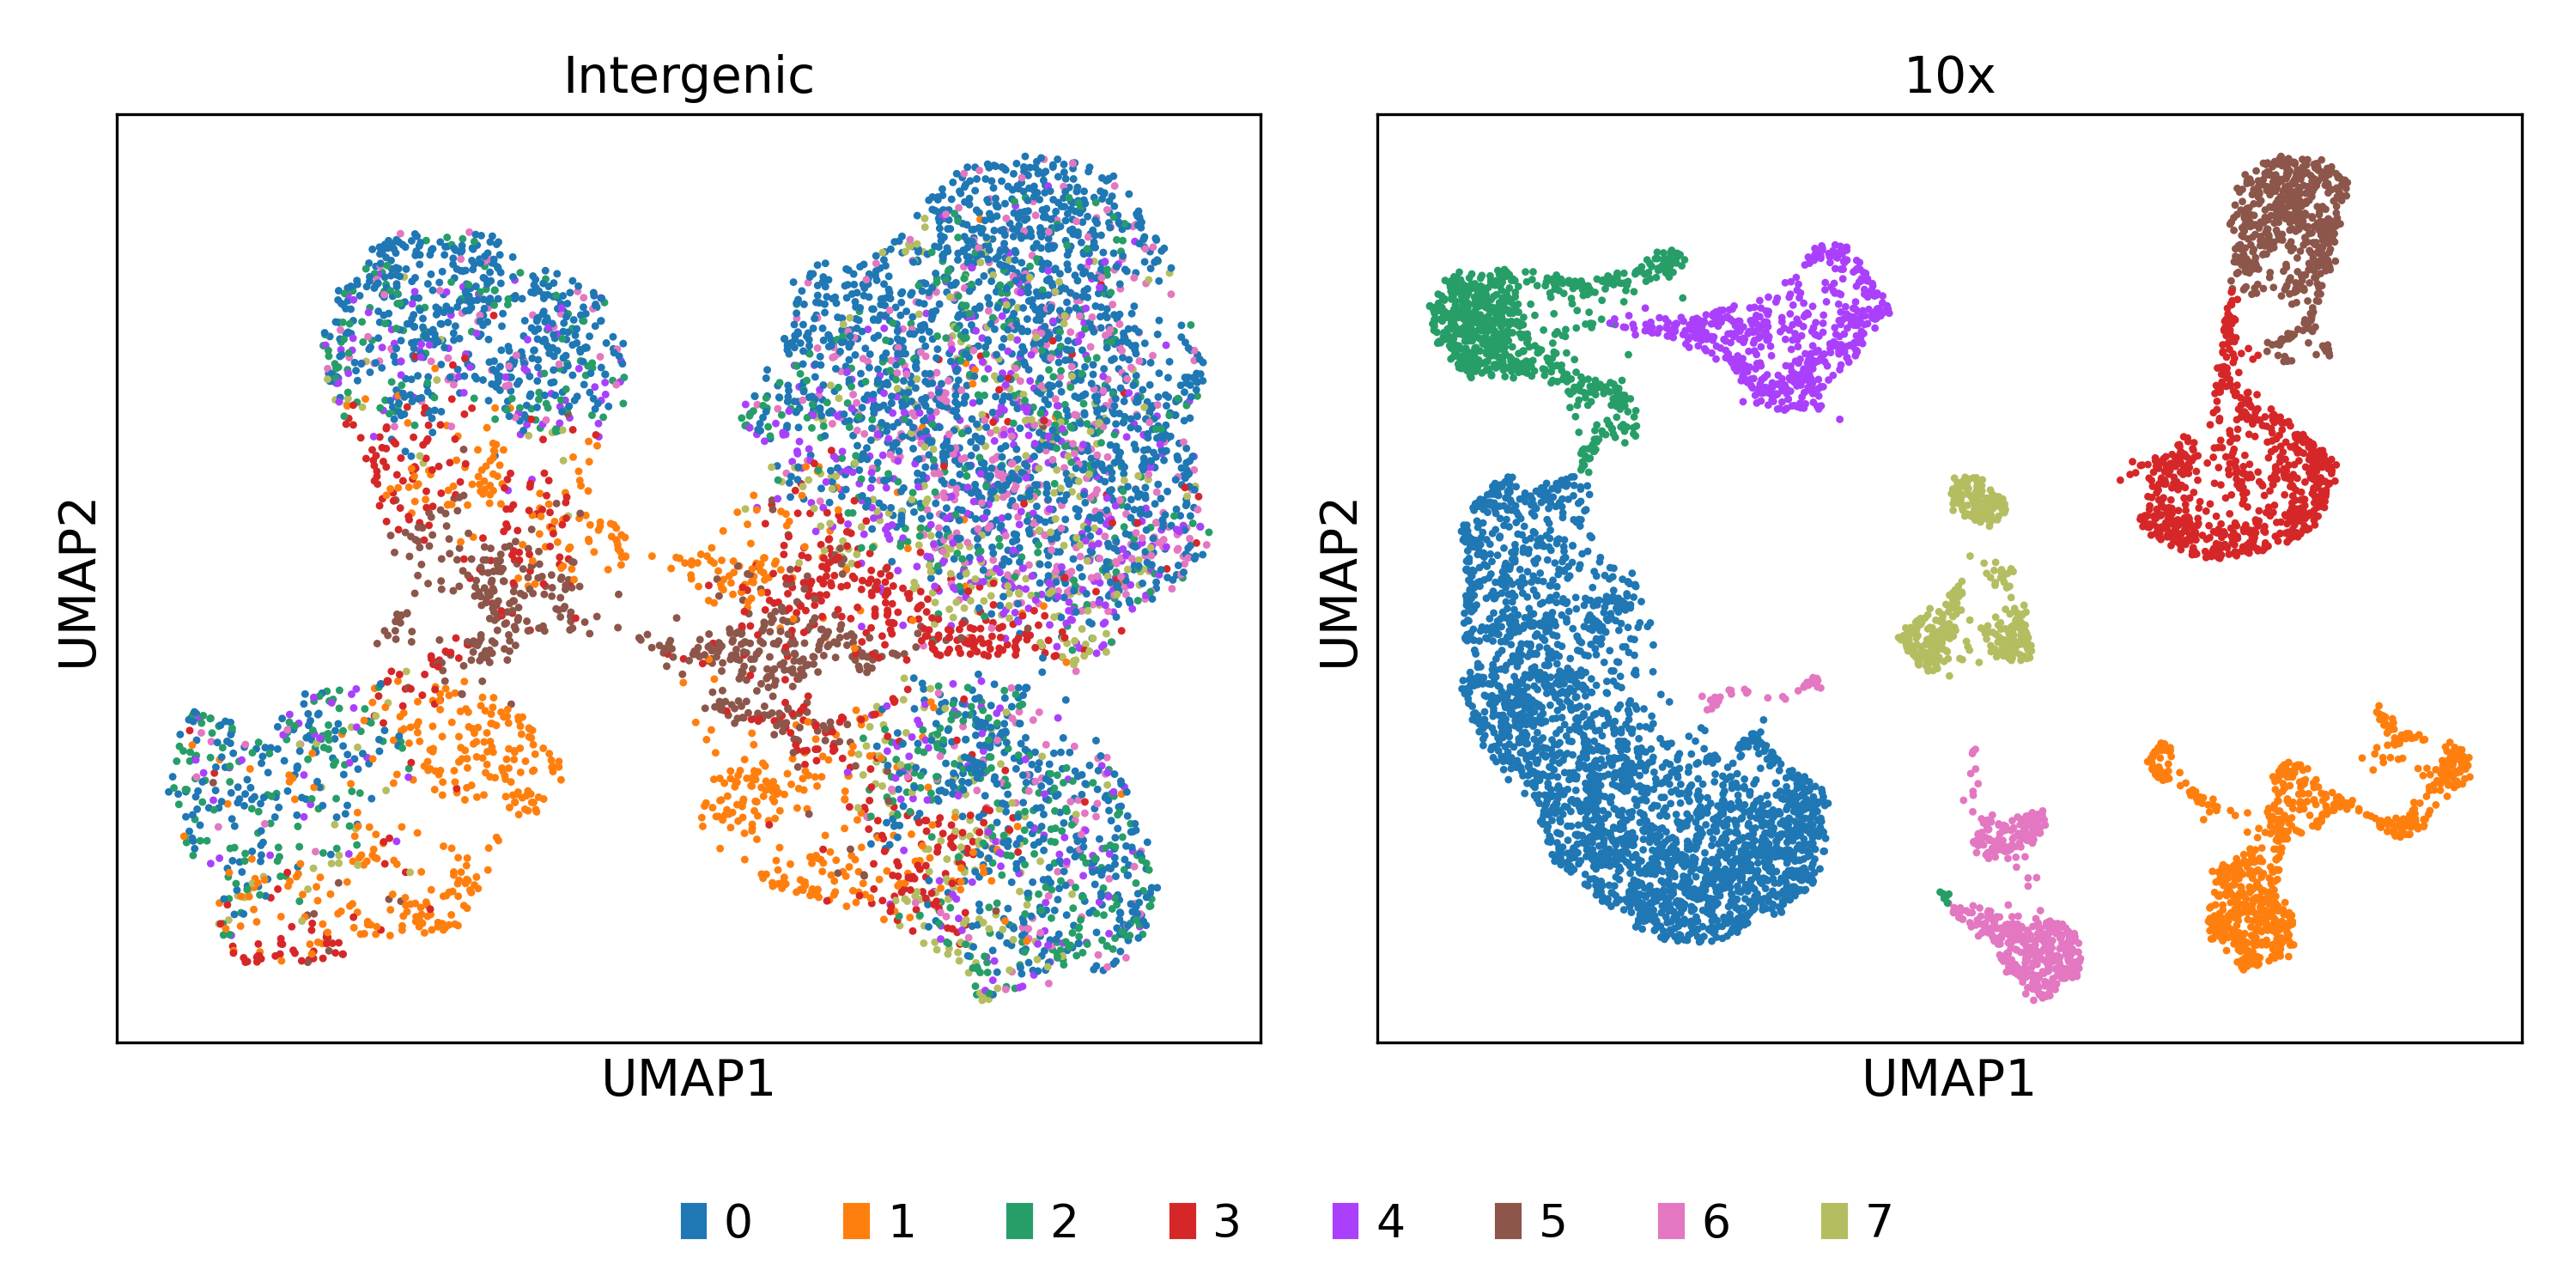
\includegraphics[width=\textwidth]{images/umaps/intergenic_10x_brain_2.png}
        \caption{10x Brain 2}
    \end{subfigure}
    \caption{Comparison of clustering using standard annotation ('10x' reference) and using only defined intergenic regions.
    As can be seen, for some samples intergenic regions are sufficient for rough clustering, for others (e.g. 'brain\_2' sample), 
    noise gives some clustering artefacts.
    Nevertheless, the clustering can be seen even in those noisy samples.}
    \label{fig:intergenicClustering}
\end{figure}

\subsection{Intergenic regions with high conservation score}

The filtering based on the conservation as described above left five intergenic regions, given in the Table \ref{tab:conservedIntergenic}.

\begin{table}[h]
    \centering
    \begin{tabular}{lccc}
        \toprule
        Name & Genomic coordinates & Conservation score & Found in samples \\
        \midrule
        INT1216 & 1:72282700-72282900 & 0.7534172617 & brain, eye\\
	INT1829 & 1:77772950-77773050 & 0.6863111111 & lung \\
	INT2199 & 6:148122550-148122750 & 0.6364459652 & brain, eye \\
	INT2208 & 5:18162950-18163100 & 0.6138651685 & PBMC (indrops) \\
	INT3636 & X:129412750-129413050 & 0.7218984354 & brain \\
        \bottomrule
    \end{tabular}
    \caption{Conserved intergenic regions not overlapping with known genes from ncbi and gencode annotations.}
    \label{tab:conservedIntergenic}
\end{table}

\subsection{Gene Predictions Tools}

61 intergenic regions overlap with predicted genes from UCSC gene prediction archive, given in the Table \ref{tab:predictionToolsIntergenic}.
Of them 44 are in the 3' end of predicted gene (good, as our datasets are generated using 3' end sequencing protocols).
Out of those 44 predicted genes, 15 are extended versions of genes present in gencode/ncbi references,
you can see an example in Figure \ref{fig:predictedExtention}.

\begin{figure}
  \centering
  \includegraphics[width=\linewidth]{images/igv/INT33.png}
  \caption{Example of gene which is predicted to have some longer transcripts than are present in the gencode and ncbi annotations.
  The intergenic region is located after the 3' end of gene DUSP1, however,
  SIB prediction tool suggest that longer transcripts should be included in the annotation of this gene.}
  \label{fig:predictedExtention}
\end{figure}


\begin{table}[h]
    \tiny
    \centering
    \begin{tabular}{lccc}
        \toprule
        Name & Genomic coordinates & Prediction tool & Overlaps with 3' region of predicted gene \\
        \midrule
	INT7 & 6:24718850-24719100 & SIB & Yes \\
	INT33 & 5:172767250-172767500 & SIB & Yes (DUSP1) \\
	INT134 & 15:41280550-41280800 & SIB & Yes (extends a bit after) \\
	INT196 & 6:89086200-89086500 & SIB & Yes (PNRC1) \\
	INT218 & 5:61409150-61409400 & SPG & No (5' end) \\
	INT285 & 10:110898200-110898550 & SIB & Yes (BBIP1) \\
	INT327 & 1:169132100-169132350 & SIB & Yes (NME7) \\
	INT347 & 14:75277700-75278000 & Gescan & No \\
	INT382 & 12:11892250-11892500 & Gescan & Yes \\
	INT386 & 6:26215200-26215450 & SIB & Yes (H2BCB?) \\
	INT438 & 4:39713300-39713600 & SIB & Yes (almost all (short) gene spanned) \\
	INT533 & 8:130110900-130111150 & SIB & Yes \\
	INT617 & 15:85733950-85734200 & SIB & Yes \\
	INT621 & 9:75148850-75149400 & SIB & Yes (OSTF1) \\
	INT651 & 1:28579100-28579350 & SIB & Yes (TRNAU1AP) \\
	INT654 & 6:34382850-34383050 & SIB & No (but short gene)\\
	INT827 & 9:94111950-94112200 & SIB & Yes \\
	INT828 & 8:133035800-133036050 & SIB & Yes (SLA) \\
	INT859 & 2:71373500-71373750 & SIB & No (slight overlap on 5' end) \\
	INT898 & 17:51190400-51190700 & SIB & Yes (extends after)\\
	INT903 & 8:22613400-22613650 & SIB & Yes \\
	INT949 & 9:111693050-111693400 & SIB & Yes \\
	INT972 & 15:64954800-64955350 & SIB & Yes \\
	INT984 & 18:63291900-63292200 & Geneid & Yes No \\
	INT1028 & 5:50414200-50414500 & SIB & Yes No \\
	INT1155 & 1:36296050-36296300 & SIB & Yes No \\
	INT1216 & 1:72282700-72282900 & SIB & Yes No \\
	INT1231 & 10:19890700-19891050 & Gescan & Yes No \\
	INT1387 & 11:63570800-63571050 & SIB & Yes No \\
	INT1402 & 5:142786700-142786950 & SIB & Yes No \\
	INT1440 & 2:235746450-235746700 & SIB & Yes No \\
	INT1445 & 9:40885650-40885900 & SIB & Yes No \\
	INT1525 & 8:11842200-11842350 & SIB & Yes No \\
	INT1548 & 7:50342700-50342950 & Gescan & Yes No \\
	INT1616 & 17:30895450-30895700 & SIB & Yes No \\
	INT1749 & 3:172333550-172333750 & SIB & Yes No \\
	INT1801 & 5:151272550-151272700 & SIB & Yes No \\
	INT1931 & 17:82522100-82522350 & SIB & Yes No \\
	INT2044 & 19:4041150-4041400 & SIB & Yes No \\
	INT2065 & 10:103606150-103606400 & SIB & Yes No \\
	INT2158 & 14:49636100-49636350 & SIB & Yes No \\
	INT2194 & 7:130521250-130521500 & SIB & Yes No \\
	INT2371 & 1:14632650-14632900 & Geneid & Yes No \\
	INT2380 & 22:33853900-33854150 & Geneid & Yes No \\
	INT2825 & 13:45300050-45300300 & Geneid & Yes No \\
	INT2979 & 4:98929350-98929600 & SIB & Yes No \\
	INT3328 & 2:184604250-184604500 & SIB & Yes No \\
	INT3429 & 17:48172750-48173150 & Augustus & Yes No \\
	INT3504 & 15:25332950-25333150 & SIB & Yes No \\
	INT3849 & 3:121432200-121432400 & SIB & Yes No \\
	INT3868 & 17:31448500-31448700 & SIB & Yes No \\
	INT4070 & 4:47430500-47430700 & SIB & Yes No \\
	INT4147 & 1:34861500-34861700 & SIB & Yes No \\
	INT4458 & 5:44820700-44820900 & SIB & Yes No \\
	INT4577 & 5:702050-702300 & SIB & Yes No \\
	INT4743 & 20:3188900-3189050 & SIB & Yes No \\
	INT4948 & 5:703250-703450 & SIB & Yes No \\
	INT5002 & 11:92232750-92232950 & SIB & Yes No \\
	INT5315 & 20:3183750-3184050 & SIB & Yes No \\
	INT5329 & 13:95603000-95603200 & SIB & Yes No \\
	INT5710 & 4:47428500-47428700 & SIB & Yes No \\
        \bottomrule
    \end{tabular}
    \caption{Intergenic regions overlapping with predicted genes from UCSC gene prediction archive.}
    \label{tab:predictionToolsIntergenic}
\end{table}


\subsection{Intergenic regions specific to some cell types}

If reads from specific intergenic region are specific for only subset of cell types present in the sample,
it is strong indication that those reads are not sequencing artefacts.
Examples of such regions can be seen in the Figure \ref{fig:intergenicSpecific}.

\begin{figure}[htbp]
    \centering
    \begin{subfigure}{0.45\textwidth}
        \centering
        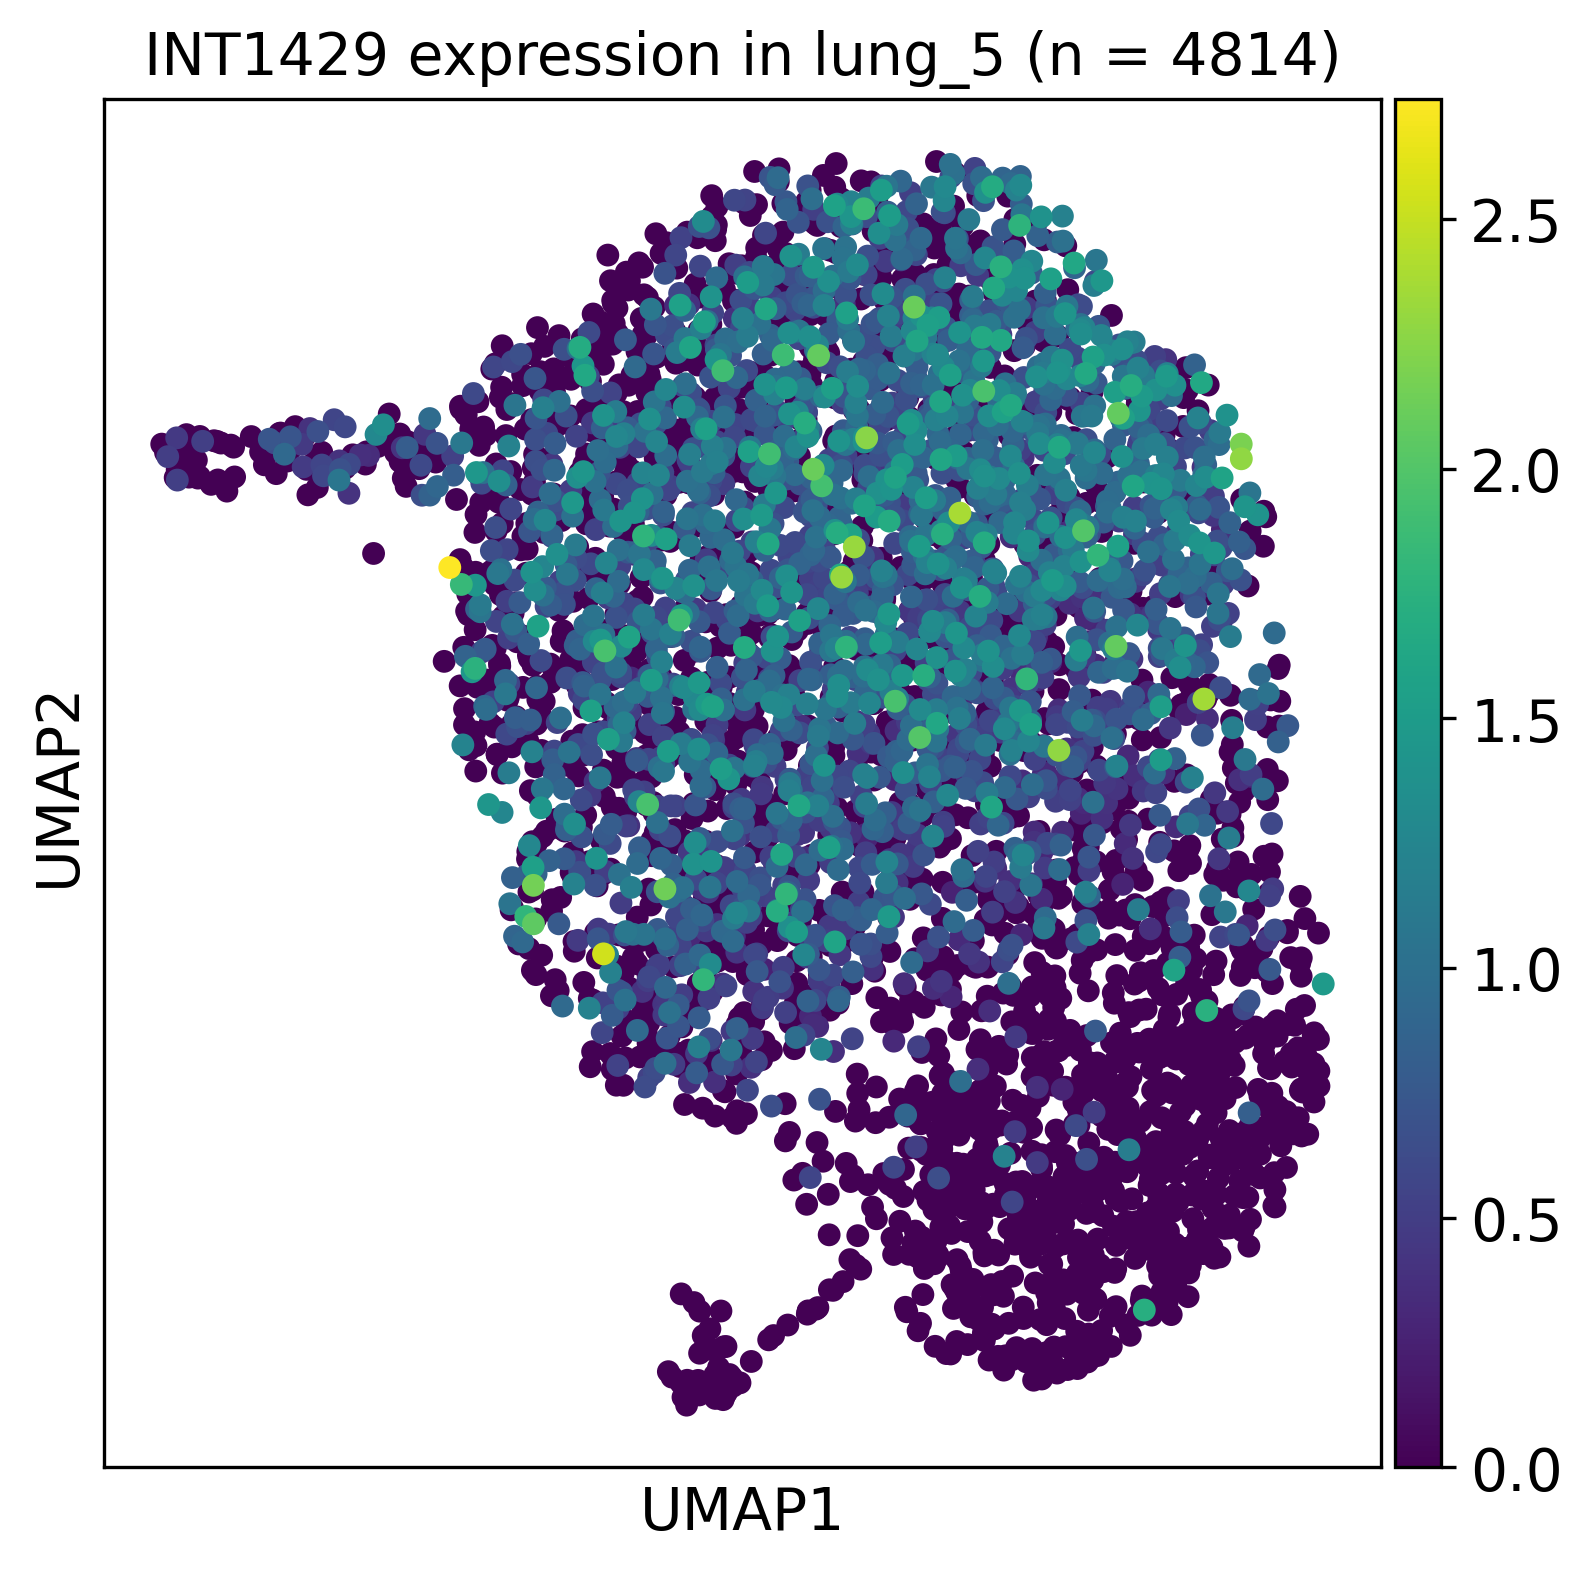
\includegraphics[width=\textwidth]{images/intergenicSpecificExamples/INT1429_lung_5.png}
        \caption{Lung 5 (INT1429)}
    \end{subfigure}
    \hfill
    \begin{subfigure}{0.45\textwidth}
        \centering
        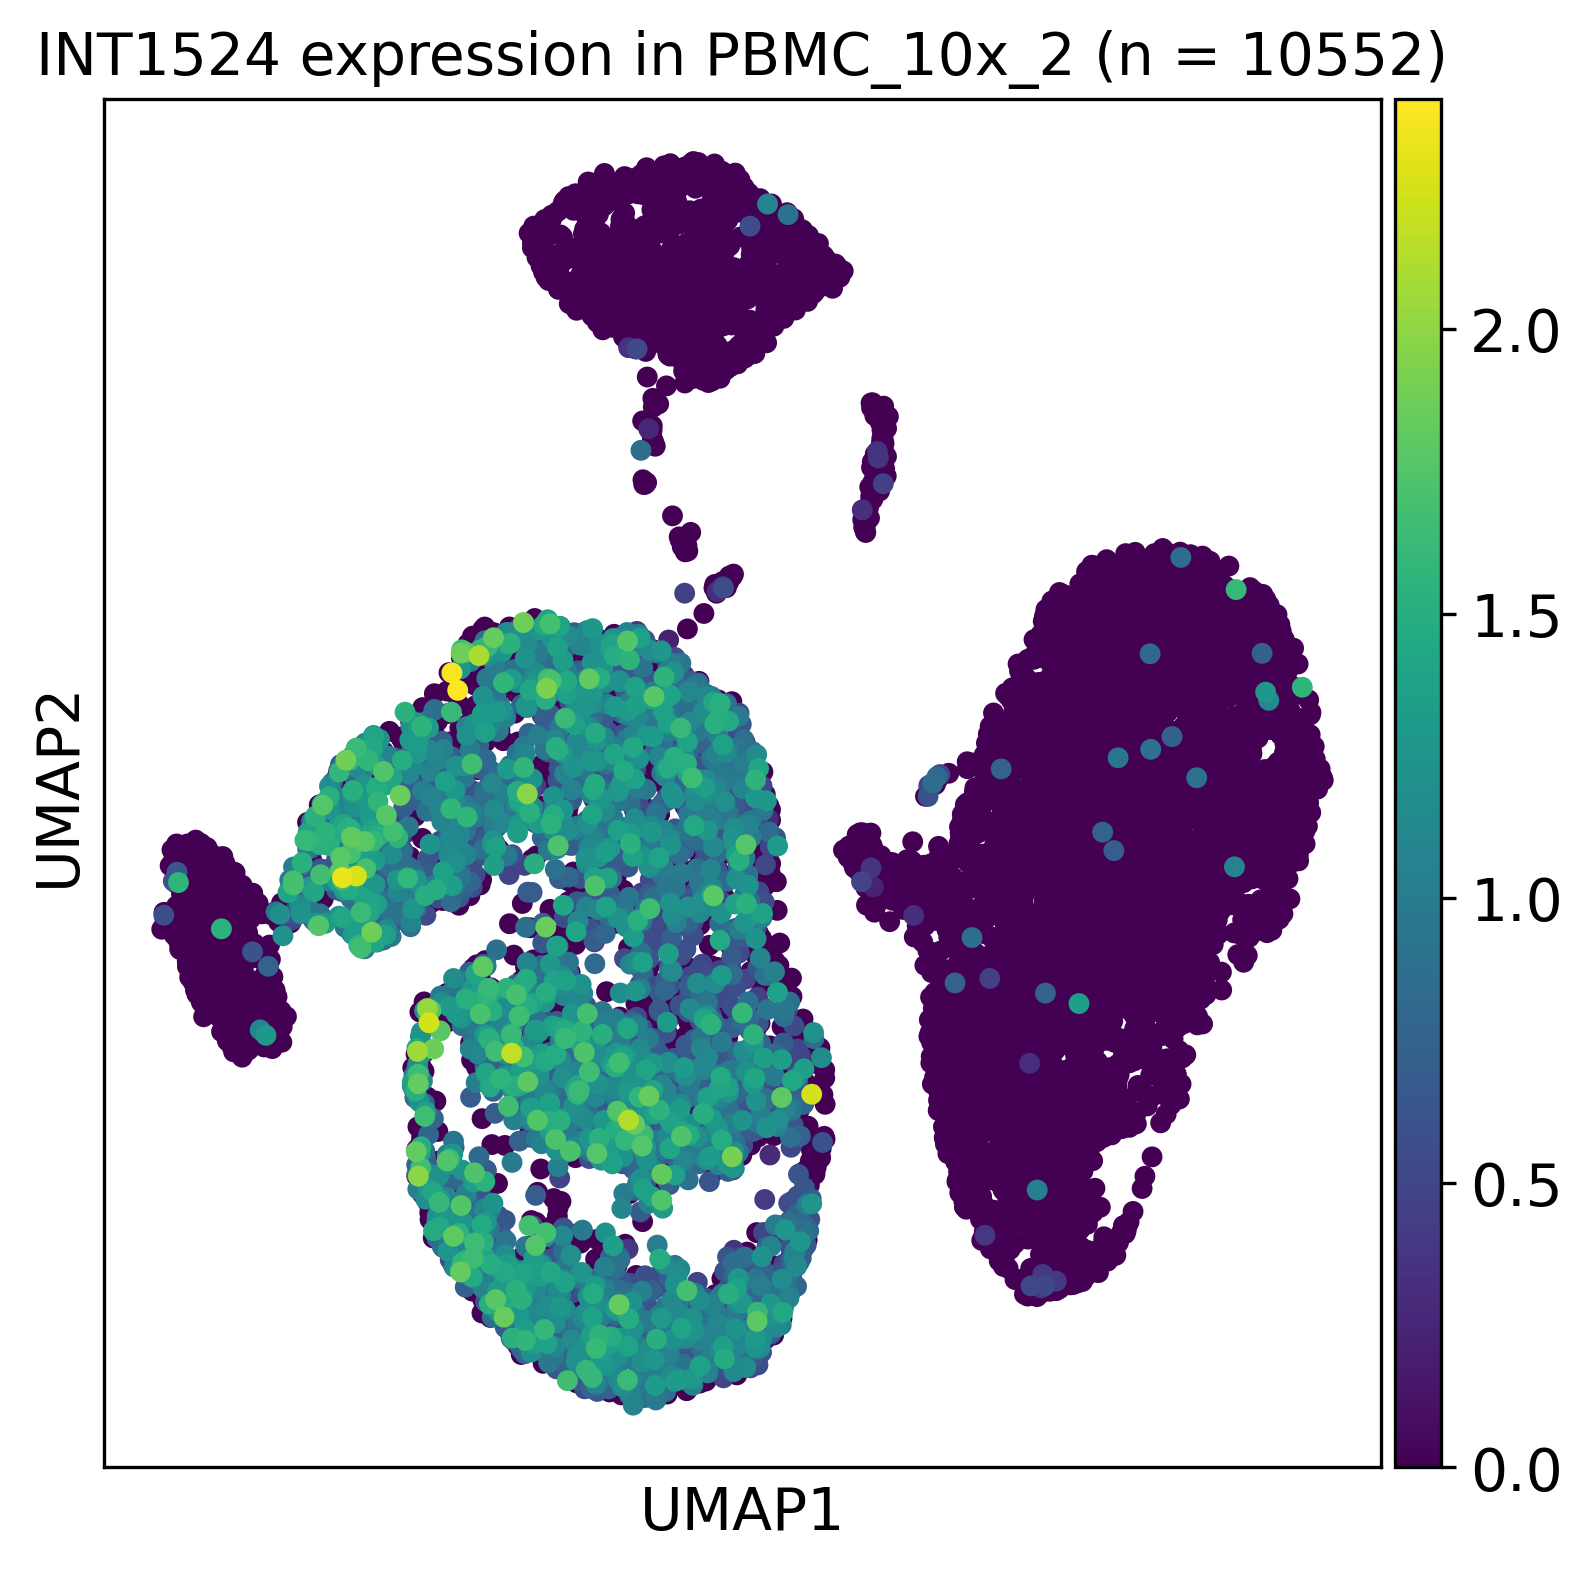
\includegraphics[width=\textwidth]{images/intergenicSpecificExamples/INT1524_PBMC_10x_2.png}
        \caption{PBMC 10x 2 (INT1524)}
    \end{subfigure}
    \vspace{0.5em}
    \begin{subfigure}{0.45\textwidth}
        \centering
        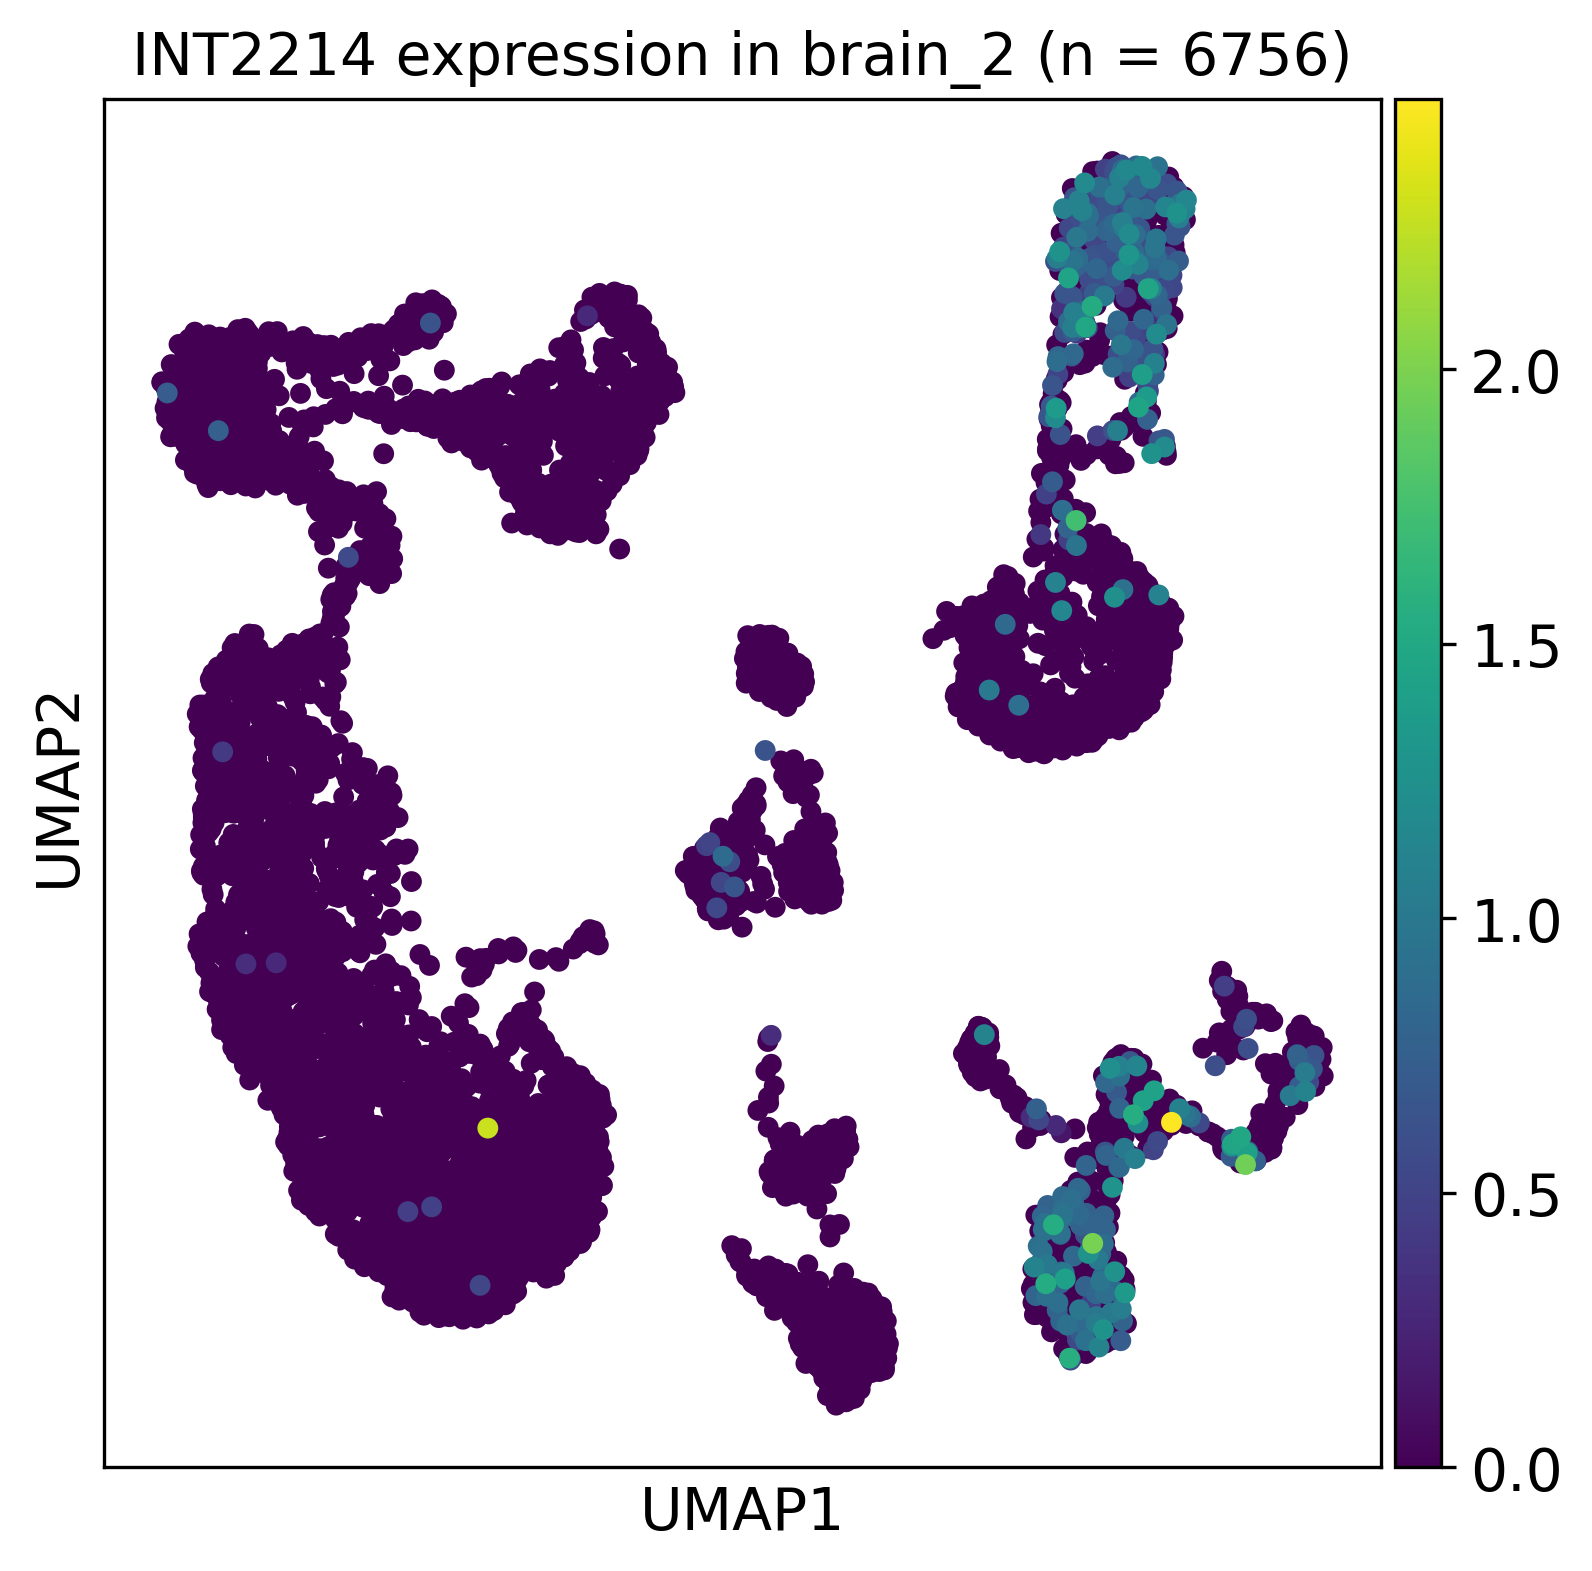
\includegraphics[width=\textwidth]{images/intergenicSpecificExamples/INT2214_brain_2.png}
        \caption{Brain 2 (INT2214)}
    \end{subfigure}
    \hfill
    \begin{subfigure}{0.45\textwidth}
        \centering
        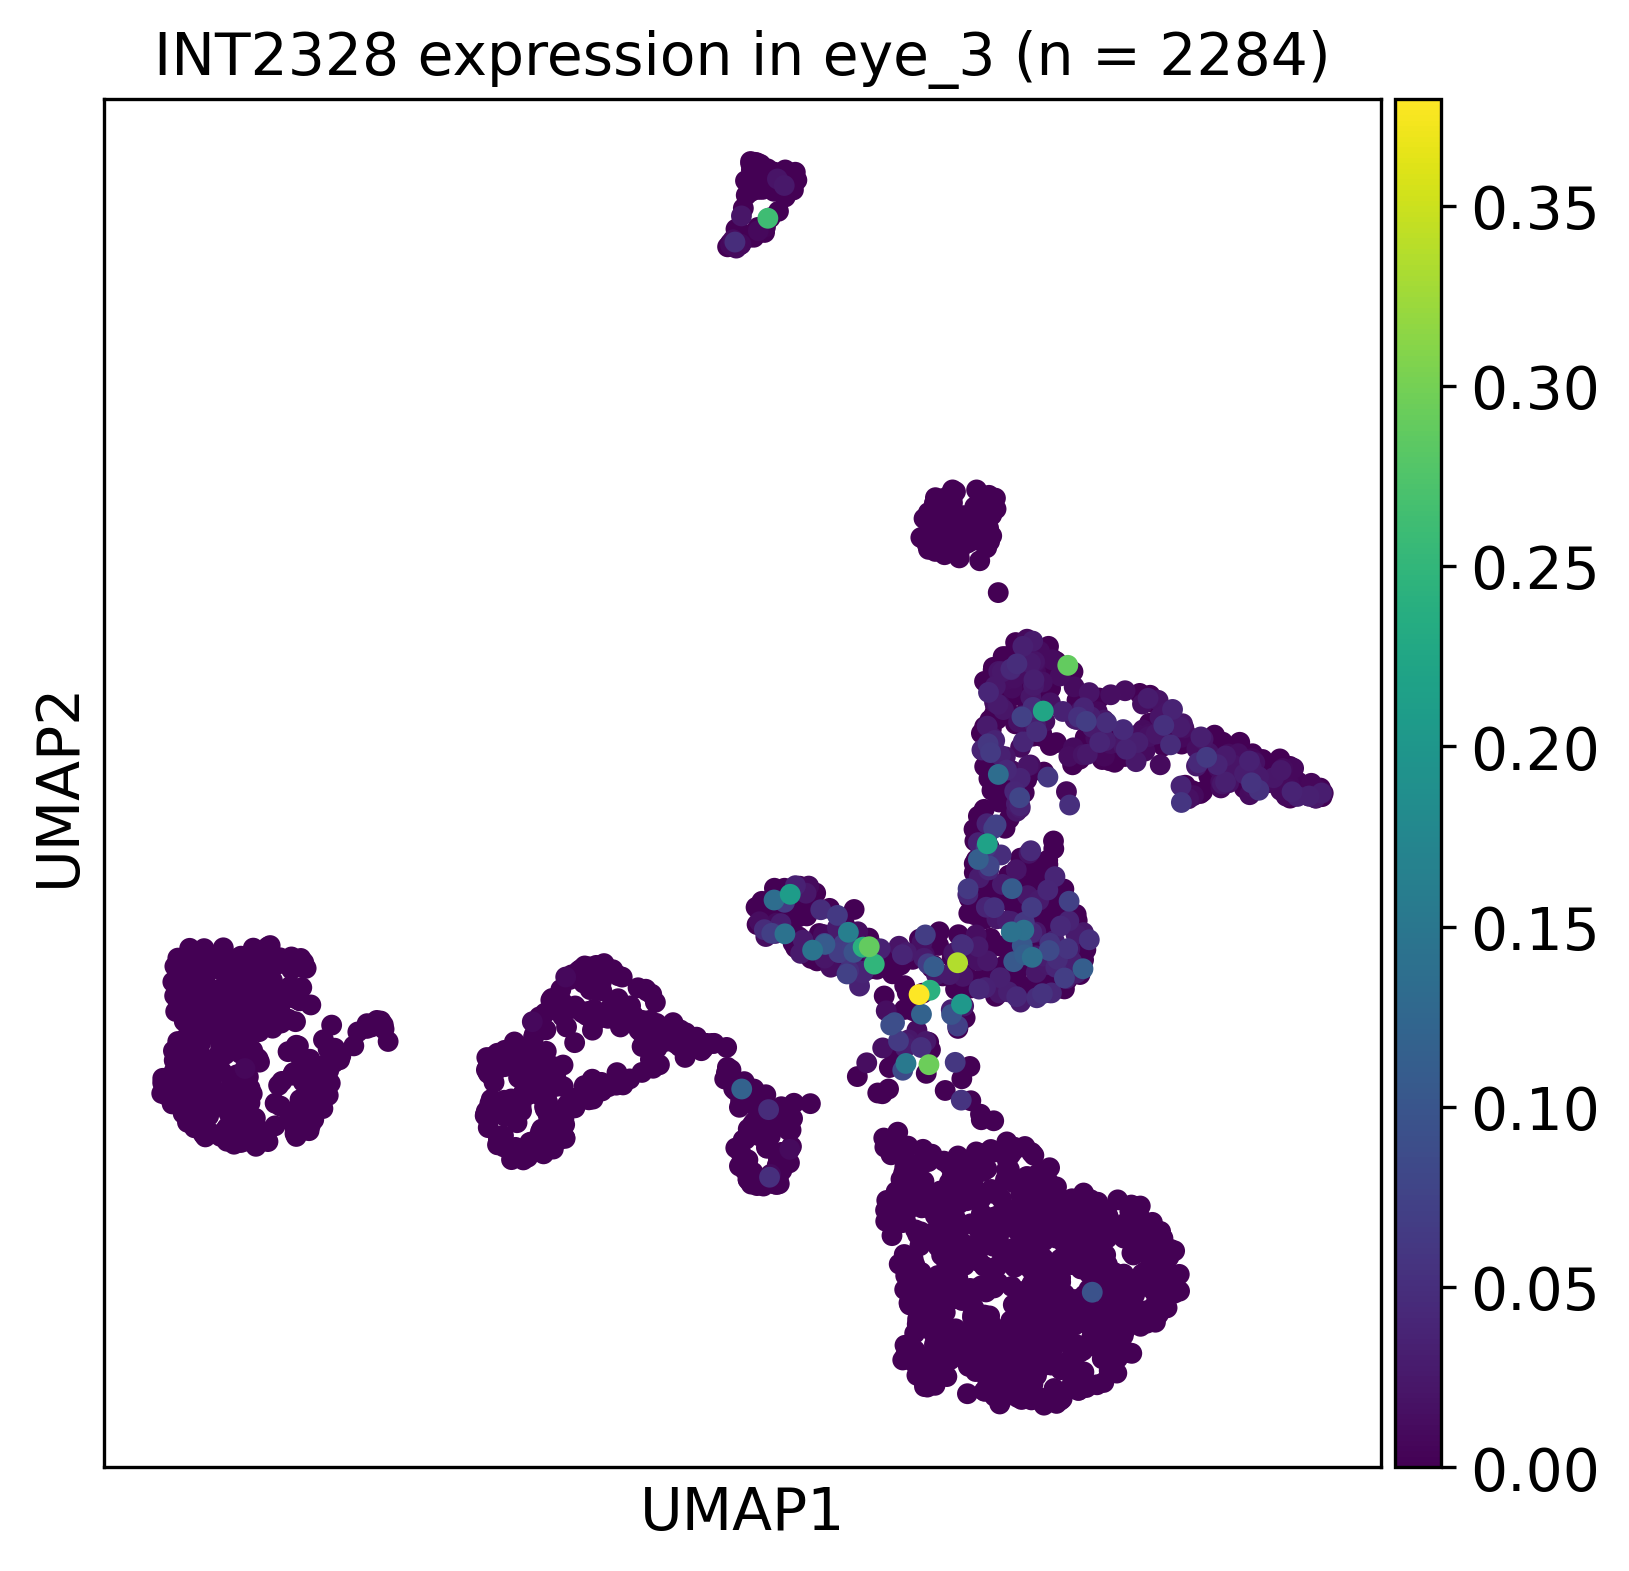
\includegraphics[width=\textwidth]{images/intergenicSpecificExamples/INT2328_eye_3.png}
        \caption{Eye 3 (INT2328)}
    \end{subfigure}
    \caption{Some examples of specificly expressed intergenic regions in various samples.}
    \label{fig:intergenicSpecific}
\end{figure}

\subsection{ATAC data}

ATAC sequencing shows open chromatin sites, which could potentially indicate that some transcription activity is happening at those sites.
Hence, checking if there are overlaps between open chromatine regions and dewfined intergenic regions could provide additional evidence of
those regions being not noise.
However, there are some caveats in this 'evidence'.
Firstly, open chromatin is mostly expected at the transcription start sites, promoter or other regulatory elements,
which are typically located in the 5' end of the gene.
Another problem is that majority of our defined regions lay on the opposite strands of known genes, while ATAC sequencing is not strand specific.
In such cases, open chromatine could be present due to the transcription of those known genes.

Out of 2590 intergenic regions, 309 intersected with ATAC intervals found from 10x PBMC ATAC data.
Out of those 309 regions, only 20 were not overlapping with genes from GENCODE or RefSeq annotations.

\subsection{Correlations}

Another aspect to check is whether expression of those intergenic regions correlate with the expression of nearby genes.
If it does, it might indicate several things:
\begin{itemize}
  \item If the region correlates with gene on the same strand:
  \begin{itemize}
    \item There might exist longer unannotated transcripts that involve those intergenic regions.
    \item The intergenic genes are involved in the same processes as the gene.
    \item They both can be transcribed by the same polymerases.
  \end{itemize}
  \item If the region correlates with gene on the oposite strand:
  \begin{itemize}
    \item The intergenic gene is involved in the same processes as the gene on the oposite strand.
    \item There happens some transcription errors that cause transcription from the opposite strand.
    \item There happens some errors in the library preparation/sequencing steps that cause template switch.
  \end{itemize}
\end{itemize}

Which of those are the case in our samples, is hard to tell.
Out of all defined intergenic regions, 86 showed Spearman correlation \textgreater 0.5 (p \textless 0.05) in at least 1 sample
(80 correlated with genes on the opposite strand, 10 with gene on the same strand, 4 with both).
Some examples can be seen in Figure \ref{fig:correlationUmaps}.

\begin{figure}[htbp]
    \centering
    \begin{subfigure}{\textwidth}
        \centering
        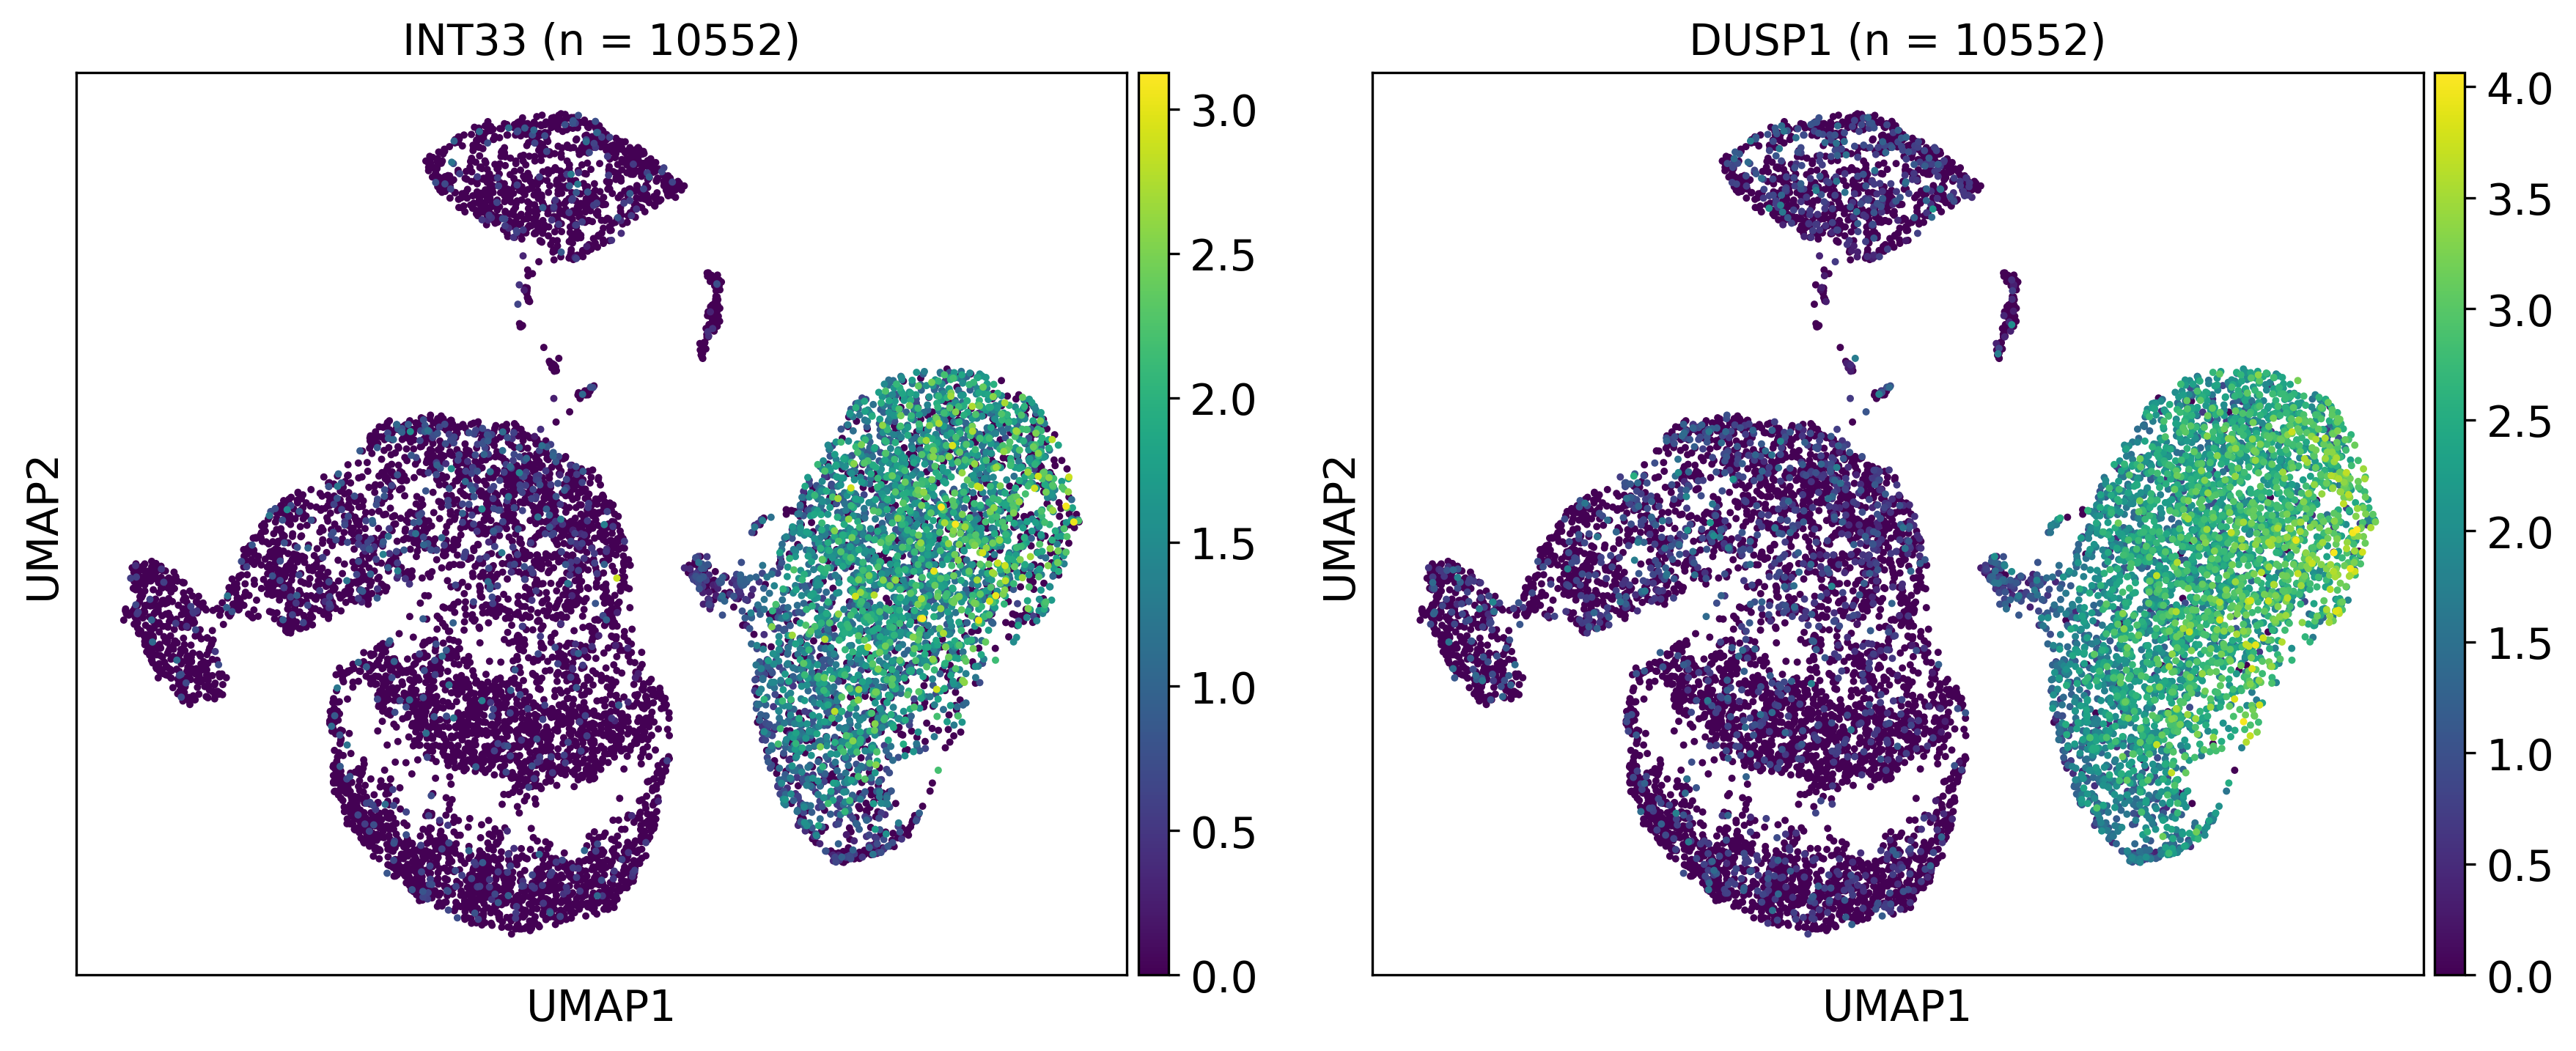
\includegraphics[width=\textwidth]{images/correlationUmaps/PBMC_10x_2_DUSP1.png}
        \caption{Umaps of INT33 and DUSP1 (Spearman correlation 0.68) of the PBMC\_10x\_2 sample, both of them are on the same strand.}
    \end{subfigure}
    \vspace{0.5em}
    \begin{subfigure}{\textwidth}
        \centering
        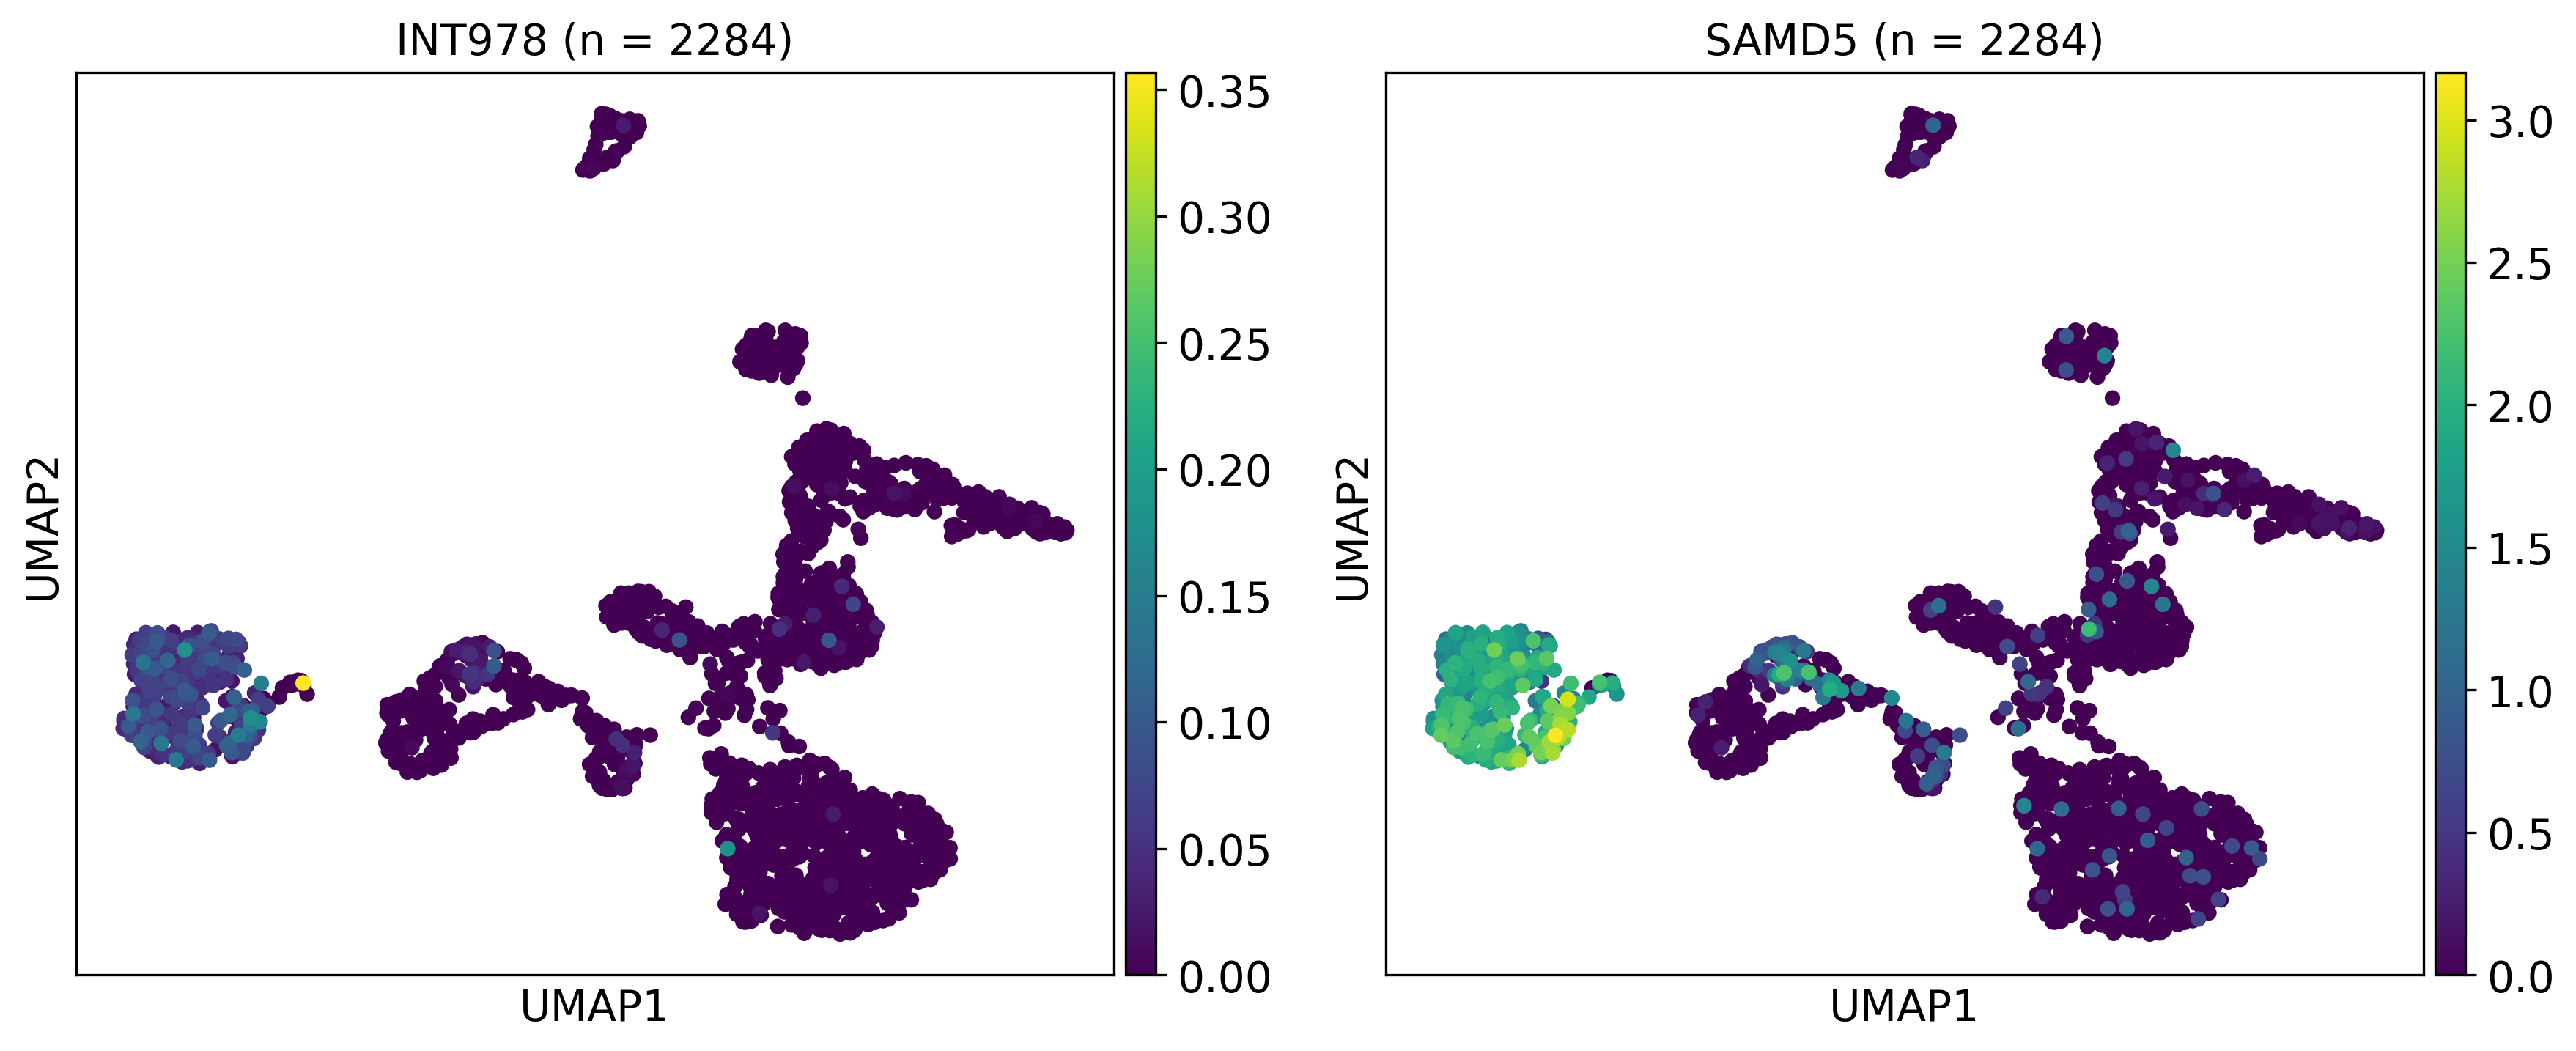
\includegraphics[width=\textwidth]{images/correlationUmaps/eye_3_SAMD5.png}
        \caption{Umaps of INT978 and SAMD5 (Spearman correlation 0.85) of the eye\_3 sample,
        intergenic region is on the opposite strand of the gene.}
    \end{subfigure}
    \caption{Correlation can be seen visually in UMAPs (colored by the normalized expression of the genes), here couple of examples given.}
    \label{fig:correlationUmaps}
\end{figure}

\fi



\iffalse

\section{Enhancing transcriptomic reference}

The enhanced transcriptomic reference allows to include those reads into downstream analysis that otherwise would be discarded.
To achieve this, we have combine data from several different transcriptomic annotations,
and additionally included in the annotation intergenic regions that contained relativelly high number of reads.

\input{"data/downstream/summaries/count_summaries/count_summary.tex"}

\subsection{Exploring unassigned reads}
Unassigned reads could come from several sources:
sequencing artefacts, genes that are not included into transcriptomic reference used, or genes that are not annotated yet.
To check, we have looked at intersections of those unassigned reads and more comprehensive annotations.
As we can see, that there are plenty of genes from more comprehensive annotations which intersect with unassigned genes,
and number of those intersecting genes correlates with sequencing depth.

\input{"data/downstream/summaries/gene_summaries/intersecting_gene_summary.tex"}

\subsection{Intergenic regions}

Observed intergenic regions can be either artefacts or be biologically meaningfull.
To check this, I have tried to cluster cells based only on the newly defined intergenic regions (see figure \ref{fig:umapComparisonIntergenic}).
While for PBMC\_indrops sample it looks as noise, for the 10x indrops samples it provides quite good clustering,
meaning that at least some of those captured intergenic regions are not sequencing artefacts.

\subsection{Enhanced Reference}

Using enhanced reference allowed us to have more captured genes in the data,
however, no significant change in clustering can be seen.

\input{"data/downstream/summaries/captured_gene_summaries/captured_gene_types_summary.tex"}

\subsection{Captured genes}

\fi
